\documentclass[a4paper]{scrreprt}
\usepackage[T1]{fontenc}
\usepackage[utf8]{inputenc}
\usepackage[ngerman]{babel}
\usepackage{graphicx}
\usepackage{subfigure}
\usepackage[official]{eurosym}
\usepackage{listings}
\usepackage{setspace}
%tabellenpackages
\usepackage{booktabs}
\usepackage{array}
\usepackage{ragged2e}
\usepackage{hyperref}
\usepackage{chngcntr} 
\counterwithout{footnote}{chapter}
%
%
% Dokumentstart
\begin{document}
\author{Josephine Reiche}
\title{Mathematische Grundlagen des Machine-/ Deep Learning}
\maketitle
\tableofcontents
\onehalfspacing
%
%
\chapter{Selbstständigkeitserklärung}
% Der Arbeit ist folgende Erklärung beizufügen:
Hiermit versichere ich, dass ich die schriftliche Hausarbeit selbstständig verfasst und keine
anderen als die angegebenen Quellen und Hilfsmittel benutzt habe. Die Stellen meiner Arbeit,
die dem Wortlaut oder dem Sinne nach anderen Werken und Quellen, einschließlich Quellen
aus dem Internet, entnommen sind, habe ich in jedem Fall unter Angabe der Quelle deutlich
als Entlehnung kenntlich gemacht. Dasselbe gilt sinngemäß für Tabellen, Karten und
Abbildungen.
% Einleitung (Motivation, Einführung in die Begriffe, Ziel der Arbeit
\chapter{Einleitung}
\section{Motivaion}
Die vorliegende Facharbeit setzt sich mit dem derzeit allgegenwärtigen Thema ``Künstliche Intelligenz (KI)'' auseinander. Alle entwickelten Länder der Welt, insbesondere aber die Technologieführer USA, China und Europa, kämpfen um die Vorherrschaft auf diesem neuen Gebiet der Informatik. Was macht dieses Thema so interessant und zukunftsrelevant, dass die Bundesregierung drei Milliarden Euro in die Entwicklung von KI-Technologien investieren möchte? Die in den letzten Jahren erzielten Fortschritte und neuen Anwendungsmöglichkeiten der KI führen zur Annahme, dass die KI in Zukunft unsere Wirtschaft und das Leben der Menschen allgemein disruptiv verändern werden. Diese Entwicklung ist mit der Einführung der Dampfmaschinen, der Stromversorgung oder dem Internet vergleichbar. Schon heute sind vielfältige Anwendungen aus dem Bereich der KI verfügbar. Beispiele dafür sind die Gesichtserkennung in Smartphones, die Google-Suche, personalisierte Werbung oder autonomes Autofahren. Viele Anwendungsbereiche der KI sind noch nicht vorhersehbar und werden mit Sicherheit alle Bereiche des Lebens erobern. Dabei lauern auch unzählige Gefahren und Probleme, die auch kritisch hinterfragt werden müssen. Das Spannende an den Technologien hinter der KI ist, dass sie auf den Grundlagen der Mathematik basieren, die für Schüler der Sekundarstufe II nachvollziehbar sind. So kann der theoretische Unterrichtsstoff in aktuelle, attraktive Experimente und Anwendungen überführt werden. 
\section{Begriffe}
Bevor die einzelnen Technologien vorgestellt werden, müssen die in dieser Arbeit verwendeten Begriffe vom allgemeinen Sprachgebrauch abgegrenzt werden. Denn was bedeutet das allgemeine Schlagwort ``künstliche Intelligenz'' genau? Zunächst kann KI als ein Teilgebiet der Mathematik bzw. der Informatik klassifiziert werden. Die theoretischen Grundlagen der KI wurden bereits in der Mitte des 20. Jahrhundert geschaffen, einige der dabei angewendeten statistischen Verfahren existierten schon vorher.
\\\\
Mit der Durchdringung des Internets in das Leben der Menschen und aller Industrien und dem sprunghaften Anstieg verfügbarer Datenmengen in Kombination mit genügend Rechenkapazitäten wurden diese Grundlagen zu neuem Leben erweckt. Der Begriff ``künstliche Intelligenz'' ist umstritten. Dies gilt auch für die Unterteilungen wie ``Machine-Learning'' oder ``Deep-Learning'', deren folgende Definition dem besseren Verständnis dienen sollen.\\\\
Die KI ist in die Bereiche Maschine-Learning (ML) und Deep-Learning (DL) sowie in Supervised-Learning und Unsupervised-Learning zu unterteilen. Beim Supervised-Learning, dem überwachten Lernen, werden Trainingsdaten mit bereits bekannten Ergebnisdaten angelernt. Das Lernen besteht dabei in einem Optimierungsproblem, nämlich eine oder mehrere Funktionen zu ermitteln, die die Eingabedaten auf die Ausgabedaten abbilden. Danach soll diese Funktion für unbekannte Eingabewerte möglichst genaue Ausgabedaten berechnen. Dabei kommen die maschinellen, also algorithmisch auf Computern berechneten, mathematischen Funktionen zum Einsatz. Das Deep-Learning bedient sich zusätzlich den Erkenntnissen der Neurologie und hat die Funktionsweise des menschlichen Gehirns zum Vorbild. Auch beim DL existieren zahlreiche Anwendungen des Supervised-Learning. Jedoch ist mittels des DL auch ein Unsupervised-Learning (unüberwachtes Lernen) sinnvoll möglich. Unsupervised-Learning Algorithmen agieren beispielsweise in einem spezifischen Umfeld und ``lernen'' durch die Veränderung ihrer Umgebung. So konnte der Google Deepmind Agent ``AlphaGo Zero'' die Strategien des Go Spiels selbständig ermitteln bzw. ``erlernen'' und nach einer nur 40 tägigen Trainingsphase gegen sich selbst, besser als wahrscheinlich jeder auf der Erde lebende Mensch spielen. Die Kombination von DL und Unsupervised-Learning kann somit erstmals als ``generelle künstliche Intelligenz'' bezeichnet werden. 
\newpage
\section{Ziel der Arbeit}
Im Folgenden wird der Weg vom Machine-Learning zum Deep-Learning anhand von Supervised-Learning Methoden nachvollzogen, um Schülern der Sekundatstufe II dieses interessante Thema vorzustellen. Dabei stehen die Anwendung und Kombination von Gelerntem auf einem verständlichen Niveau im Vordergrund. Die Darstellung mathematischer Probleme, deren Überführung in Algorithmen und Programmcode sollen den praktischen Nutzen des Unterrichtstoffes illustrieren. Einige notwendige Voraussetzungen, z.B. die Grundlagen von Vektoren-, Matrizen- und Differentialrechnung werden vorausgesetzt. Die algorithmischen Umsetzungen sind in Python 3 implementiert und unter https://github.com/josephinereiche abrufbar.
% Lineare Regression
\chapter{Regression}
\section{Lineare Regression}
\subsection{Einfache Lineare Regression}
Regression bezeichnet in der Mathematik statistische Analysemethoden, die Beziehungen einer oder mehrerer abhängigen Variablen modellieren. Im Kontext des Machine-Learning ist die hier vorgestellte lineare Regression dem Supervised-Learning zuzuordnen, das heißt, sie basiert auf vorgegebenen Eingabe- und Ausgabedaten. Die Ergebnisse der linearen Regression sind diskrete Werte z.B. Geldwerte, Quadratmeter.\\\\
Die lineare Regression ist eine statistische Methode, um die Daten aus einer Stichprobe oder einem Experiment durch eine angenommene lineare Funktion (Hypothese) zu beschreiben.
%(https://learnattack.de/mathe/lineare-regression)\\\\
Zur bessern Veranschaulichung der zu Grunde liegenden Prinzipien werden im folgenden Abschnitt zunächst nur Funktionen mit einer abhängigen Variablen $x$ betrachtet. Dabei soll gelten: \\
X - Menge aller Eingabewerte\\
Y - Menge aller Ausgabewerte\\
%$m$ - Anzahl der Datensätze (Elemente von X und Y)\\
%$n$ - Anzahl der abhängigen Variablen\\
$i$ - $i$'tes Element von X, Y
$x_i \in X$\\
$y_i \in Y$\\
Die Hypothese ist eine Funktion der Form:\\\\
$h_{\theta}(x)=\theta_{0}+\theta_{1}*x_{1}$ \\\\
Das allgemeine Vorgehen bei der linearen Regression lässt sich durch folgenden Ablauf beschreiben. Eine möglichst große Menge von Eingabedaten und dazugehörigen Ausgabedaten wird in zwei Gruppen eingeteilt. Die erste Gruppe enthält ca. 80\% der Daten und wird zum Training der gesuchten linearen Funktionsparameter ${\theta}$ genutzt. Nach dem Training werden die übrigen Daten als Verifikationsdaten auf die ermittelte Funktion angewendet und die Ergebnisse dieser Funktion mit den bekannten Ausgabedaten verglichen (vgl. Abbildung Modell).
\footnote{Andrew Ng - YouTube Video- Lecture 2.1- Linear Regression With One Variable | Model Representation}
\footnote{Jannis Seemann- Udemy Kurs Machine Learning von A-Z - Section 5- Lineare Regression Teil 1}
%
\begin{figure}[h]
\centering
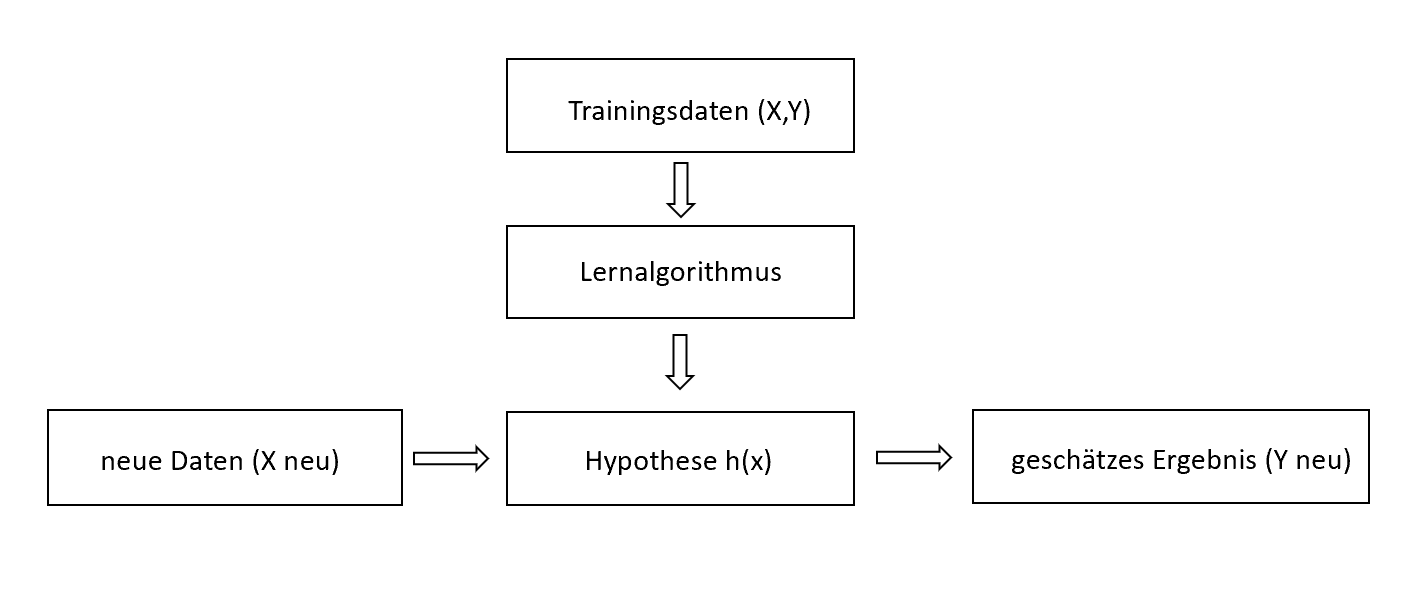
\includegraphics[scale=.75]{Abbildungen/Lineare_Regression_00}
\label{Lernmodell}
\caption{Modell}
\end{figure}
\\\\
Folgend werden die Verfahren zur Ermittlung der linearen Funktion vorgestellt.\newline
\begin{enumerate}
\item Graphische Verfahren
\newline
Hier werden die ermittelten Messwerte in einem Koordinatensystem abgebildet. Dies kann mittels eines Geometrieprogramms oder dem Schultaschenrechner durchgeführt werden. Anschließend wird eine lineare Funktion manuell im Koordinatensystem verschoben und die Abstände von den Punkten zu der Funktion nach Augenmaß minimiert. Die Parameter der gewählten linearen Funktion können dann übernommen werden. In den Abbildungen sind die Abstände zwischen den tatsächlichen Punkten und der Funktionsgerade am entsprechenden ${x}$-Wert durch Strecken angegeben. Je länger die Strecke, desto größer der Fehler, desto geringer die Eignung der Funktion als Modell. Die folgende Abbildung zeigt eine ungünstige und eine perfekte grafische Lösung des Modells.
\footnote{Andrew Ng- YouTube Video- Lecture 2.1- Linear Regression With One Variable | Model Representation}
\footnote{Jannis Seemann- Udemy Kurs Machine Learning von A-Z - Section 5- Lineare Regression Teil 2}
%
\begin{figure}[htbp]
\centering
%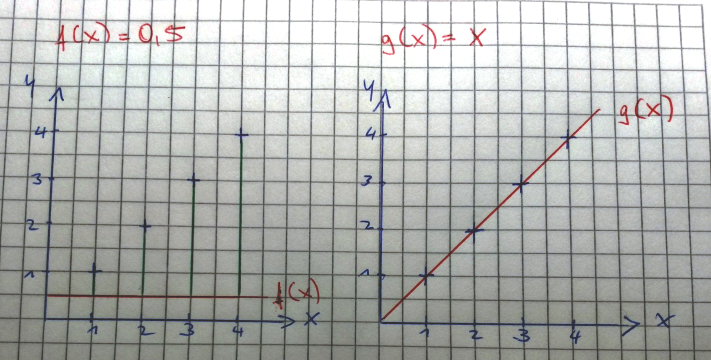
\includegraphics[scale=.5]{Abbildungen/Lineare_Regression/GrafikVerfahren}
\subfigure[Fehlerabstand]{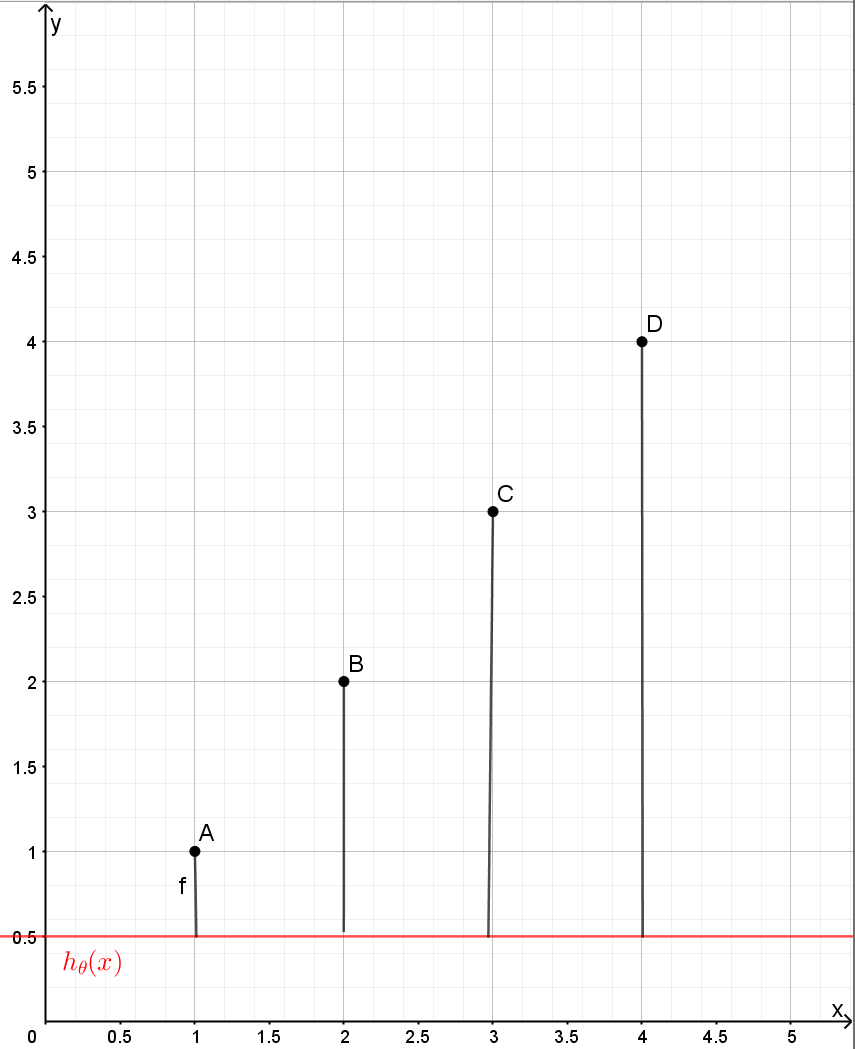
\includegraphics[scale=.5]{Abbildungen/Lineare_Regression_2}}
\subfigure[Ideallösung]{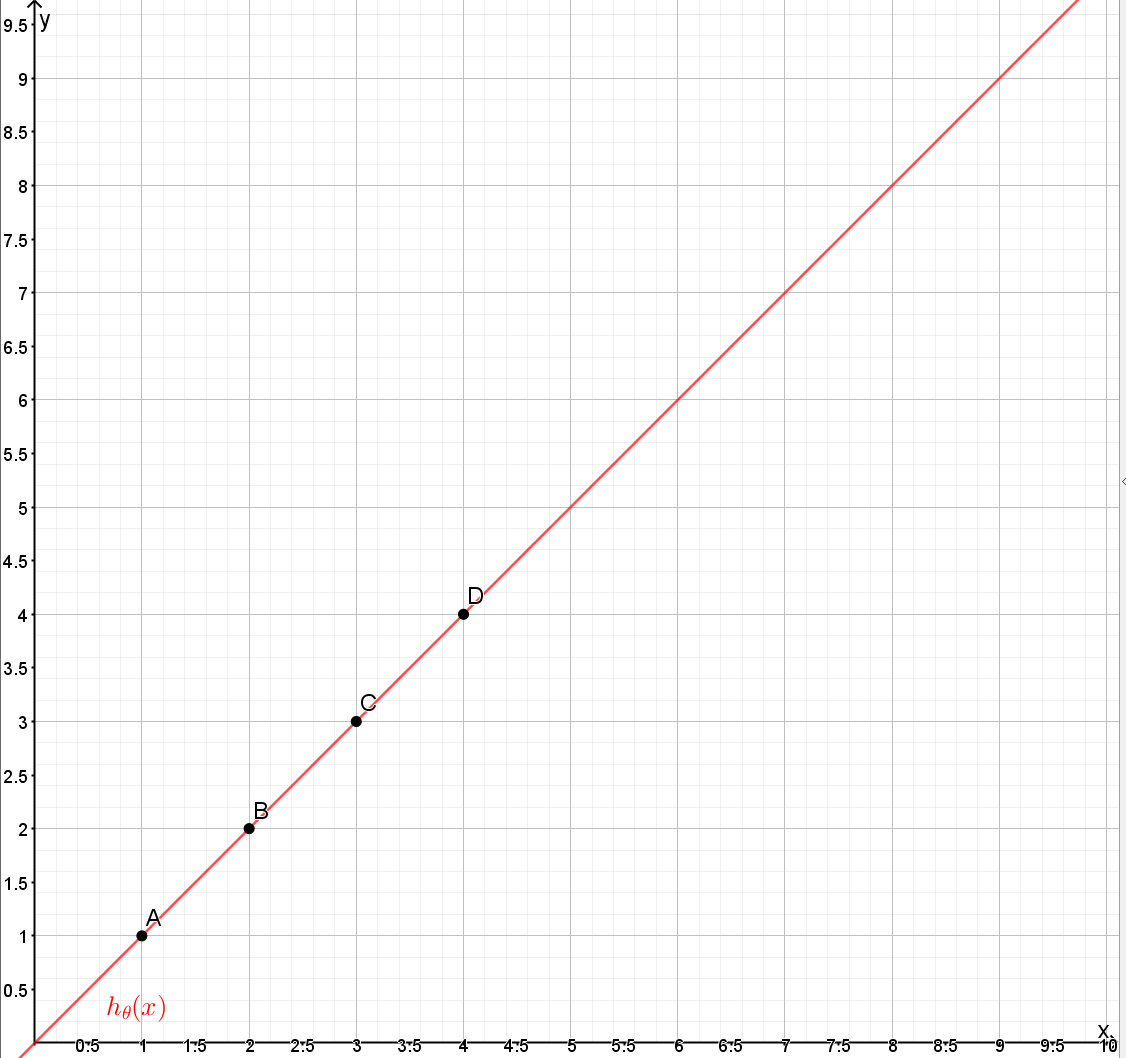
\includegraphics[scale=.5]{Abbildungen/Lineare_Regression_1}}
%\label{Abb:Lösungen}
\caption{grafische Lösungen}
\end{figure}
\newpage
\item Manuelle Berechnungen\newline
Die lineare Regression kann, besonders bei überschaubarer Anzahl von Datensätzen (n), händisch bestimmt werden. Zunächst wird der Korrelationskoeffizient r, mit der Formel:
$r= \frac{\sum (x_i-\bar{x})*(y_i-\bar{y})}{\sqrt{\sum (x_i-\bar{x})^{2}*(y_i-\bar{y})^{2}}}$,
wobei $\bar{x}$ (entsprechend $\bar{y}$) das arithmetische Mittel nach $\frac{1}{n}*\sum_{i=1}^{n} x_i$
ist, berechnet. Danach wird die Steigung $\theta_{1}$ der linearen Funktion ermittelt:\newline
$\theta_{1}= r*\frac{S_{y}}{S_{x}}$\newline
Diese Formel enthält die Standardabweichung von y und x, die wie folgt bestimmt werden:\newline
$S_{y}= \sqrt{\frac{\sum (y-\bar{y})^{2}}{n-1}}$\newline
$S_{x}= \sqrt{\frac{\sum (x-\bar{x})^{2}}{n-1}}$\newline
Zuletzt wird die Verschiebungskonstante $\theta_{0}$ durch einfaches Umstellen berechnet:\newline
%Verschiebungskonstante alternative Bezeichnung ist Ordinatenabschnitt oder y-Achsenabschnitt?
$\theta_{0}=\bar{y}-\theta_{1}*\bar{x}$\newline
Somit sind alle Parameter für die Funktion $h_{\theta}(x)=\theta_{0}+\theta_{1}*x_{1}$ bestimmt.\newline
Die folgende Tabelle enthält Beispieldaten für den Verkaufspreis einer Wohnung, der in diesem Beispiel nur von der Wohnungsgröße in $m^{2}$ abhängt.
\footnote{Jannis Seemann- Udemey Kurs- Machine Learning von A-Z- Section 5- Python: Daten einlesen und Grafik einzeichnen}
\newpage
\begin{table}
	\centering
	\refstepcounter{table}
	\label{Manuelle Regression}
\begin{tiny}
\begin{tabular}{lllllll}
\toprule
\textbf{A} in $m^{2}$ & \textbf{Preis} in \euro{} & $x_i-\bar{x}$ & $y_i-\bar{y}$ & $(x_i-\bar{x})*(y_i-\bar{y})$ & $(x_i-\bar{x})^{2}$ & $(y_i-\bar{y})^{2}$  \\
\midrule
70                    & 351000                 & 70                  & 351000              & 24570000                                    & 4900                    & 1,23201E+11             \\
72                    & 390000                 & 72                  & 390000              & 28080000                                    & 5184                    & 1,521E+11               \\
91                    & 473000                 & 91                  & 473000              & 43043000                                    & 8281                    & 2,23729E+11             \\
58                    & 282000                 & 58                  & 282000              & 16356000                                    & 3364                    & 79524000000             \\
49                    & 300000                 & 49                  & 300000              & 14700000                                    & 2401                    & 90000000000             \\
50                    & 286000                 & 50                  & 286000              & 14300000                                    & 2500                    & 81796000000             \\
48                    & 228000                 & 48                  & 228000              & 10944000                                    & 2304                    & 51984000000             \\
33                    & 181000                 & 33                  & 181000              & 5973000                                     & 1089                    & 32761000000             \\
61                    & 308000                 & 61                  & 308000              & 18788000                                    & 3721                    & 94864000000             \\
51                    & 289000                 & 51                  & 289000              & 14739000                                    & 2601                    & 83521000000             \\
78                    & 414000                 & 78                  & 414000              & 32292000                                    & 6084                    & 1,71396E+11             \\
70                    & 358000                 & 70                  & 358000              & 25060000                                    & 4900                    & 1,28164E+11             \\
35                    & 165000                 & 35                  & 165000              & 5775000                                     & 1225                    & 27225000000             \\
81                    & 397000                 & 81                  & 397000              & 32157000                                    & 6561                    & 1,57609E+11             \\
70                    & 352000                 & 70                  & 352000              & 24640000                                    & 4900                    & 1,23904E+11             \\
47                    & 239000                 & 47                  & 239000              & 11233000                                    & 2209                    & 57121000000             \\
55                    & 322000                 & 55                  & 322000              & 17710000                                    & 3025                    & 1,03684E+11             \\
70                    & 376000                 & 70                  & 376000              & 26320000                                    & 4900                    & 1,41376E+11             \\
89                    & 499000                 & 89                  & 499000              & 44411000                                    & 7921                    & 2,49001E+11             \\
68                    & 383000                 & 68                  & 383000              & 26044000                                    & 4624                    & 1,46689E+11             \\
42                    & 229000                 & 42                  & 229000              & 9618000                                     & 1764                    & 52441000000             \\
93                    & 424000                 & 93                  & 424000              & 39432000                                    & 8649                    & 1,79776E+11             \\
54                    & 256000                 & 54                  & 256000              & 13824000                                    & 2916                    & 65536000000             \\
52                    & 256000                 & 52                  & 256000              & 13312000                                    & 2704                    & 65536000000             \\
72                    & 363000                 & 72                  & 363000              & 26136000                                    & 5184                    & 1,31769E+11             \\
62                    & 328000                 & 62                  & 328000              & 20336000                                    & 3844                    & 1,07584E+11             \\
65                    & 331000                 & 65                  & 331000              & 21515000                                    & 4225                    & 1,09561E+11             \\
98                    & 465000                 & 98                  & 465000              & 45570000                                    & 9604                    & 2,16225E+11             \\
39                    & 273000                 & 39                  & 273000              & 10647000                                    & 1521                    & 74529000000             \\
50                    & 215000                 & 50                  & 215000              & 10750000                                    & 2500                    & 46225000000             \\
62                    & 287000                 & 62                  & 287000              & 17794000                                    & 3844                    & 82369000000             \\
45                    & 207000                 & 45                  & 207000              & 9315000                                     & 2025                    & 42849000000             \\
11                    & 7000                   & 11                  & 7000                & 77000                                       & 121                     & 49000000                \\
60                    & 328000                 & 60                  & 328000              & 19680000                                    & 3600                    & 1,07584E+11             \\
60                    & 282000                 & 60                  & 282000              & 16920000                                    & 3600                    & 79524000000             \\
74                    & 322000                 & 74                  & 322000              & 23828000                                    & 5476                    & 1,03684E+11             \\
64                    & 305000                 & 64                  & 305000              & 19520000                                    & 4096                    & 93025000000             \\
56                    & 317000                 & 56                  & 317000              & 17752000                                    & 3136                    & 1,00489E+11             \\
71                    & 406000                 & 71                  & 406000              & 28826000                                    & 5041                    & 1,64836E+11             \\
40                    & 225000                 & 40                  & 225000              & 9000000                                     & 1600                    & 50625000000             \\
76                    & 407000                 & 76                  & 407000              & 30932000                                    & 5776                    & 1,65649E+11             \\
88                    & 443000                 & 88                  & 443000              & 38984000                                    & 7744                    & 1,96249E+11             \\
55                    & 294000                 & 55                  & 294000              & 16170000                                    & 3025                    & 86436000000             \\
60                    & 277000                 & 60                  & 277000              & 16620000                                    & 3600                    & 76729000000             \\
79                    & 393000                 & 79                  & 393000              & 31047000                                    & 6241                    & 1,54449E+11             \\
109                   & 576000                 & 109                 & 576000              & 62784000                                    & 11881                   & 3,31776E+11             \\
51                    & 254000                 & 51                  & 254000              & 12954000                                    & 2601                    & 64516000000             \\
48                    & 263000                 & 48                  & 263000              & 12624000                                    & 2304                    & 69169000000             \\
25                    & 101000                 & 25                  & 101000              & 2525000                                     & 625                     & 10201000000             \\
88                    & 426000                 & 88                  & 426000              & 37488000                                    & 7744                    & 1,81476E+11             \\
\bottomrule
\end{tabular}
\end{tiny}	
\end{table}
%
Aus der Tabelle lassen sich folgende Werte berechnen:\\\\
$\bar{x}$= 61,9; $\bar{y}$= 317060\\\\
$r= \frac{1073115000}{\sqrt{209685*5,53052E+12}}=0,961018288$\\\\
$S_{y}= \sqrt{\frac{5,04163 E+11}{50-1}}=101434,8912$\\\\
$S_{x}= \sqrt{\frac{18104,5}{50-1}}=19,22185194$\\\\
$\theta_{1}= 0,961018288*\frac{101434,8912}{19,22185194}=5071,352426$\\\\
$\theta_{0}=317060-5071,352426*61,9=3143,284819$\\\\
Der Anstieg der durch die Regression ermittelten Funktion beträgt 5071,352426 und die Verschiebungskonstante ist 3143,284819.
%
%Hier ein Beispiel eintragen für Training und Vorraussage.
%
Der Wert einer fiktiven Wohnung mit 100$m^2$ beträgt demnach 3143,284819 + 5071,352426 * 100 = 510.278,53 Euro.\\\\
\item Algorithmische Berechnung\\\\
Die vorgestellte Methode der manuellen Berechnung der Funktionsparameter ist nur für kleinere Datensätze und wenige, hier eine abhängige Variable ${x}$ praktikabel. In der Praxis werden jedoch möglichst große Datenmengen mit hunderten oder tausenden Abhängigen verwendet, deren Parameter bestimmt werden sollen. Dazu ist ein algorithmisches Vorgehen notwendig, das hier anhand des einfachen bereits eingeführten Beispiels erläutert wird. Dabei werden die in vielen Bereichen des ML/DL genutzten Verfahren wie die Kostenfunktion (Cost-Function), der Gradientenabstieg (Gradient-Descent) und die Lernrate eingeführt.\\\\
Kostenfunktion (Cost function)\\\\
Die Kostenfunktion gibt ein Maß an, das die Fähigkeit des Modells, die Relation zwischen X und Y zu bestimmen, beschreibt. Mathematisch formuliert:\\\\
$J(\theta_{0},\theta_{1})=\frac{1}{n}\sum_{i=0}^{n}(y_{i}-(\theta_{0}+\theta_{1}*x_{i}))^{2}$\\\\
%https://ml-cheatsheet.readthedocs.io/en/latest/linear_regression.html#cost-function
%Quelle gibt N im Bruch statt n an? Habe mich erstmal für den n entschieden.
%Gute Erklärung https://math.stackexchange.com/questions/2433022/the-cost-function-derivation-in-andrew-ng-machine-learning-course
wobei $(\theta_{0}+\theta_{1}*x_i)$ die Vorhersage für den Wert an der Stelle $x_i$ und $y_i$ der tatsächliche Ergebniswert für $x_i$ ist. Die Differenz ist der Abstand beziehungsweise der Fehler der Regressionsgeraden bezüglich $y_i$. Zur Berechnung des Fehlers (den Kosten) können verschiedene Abstandsnormen angewendet werden. Hier wird der Euklidische Abstand angewendet, unter anderem um negative Ergebnisse für den Fehler auszuschließen und die Funktion differenzierbar zu gestalten.
%weitere Erkenntnis: Udemy Intuition Geogebra Beispiel Konstante Funktion, nicht quadrierte Abstände führen zu beliebig vielen Lösungen, möglicherweise keine Ableitung möglich? Kein Minimum? 
Die ermittelten Fehler werden summiert und durch die Anzahl der Datensätze geteilt, wodurch der mittlere Fehler (mittlerer Abstand) berechnet wird. Ziel ist es nun, den mittleren Fehler und somit die Kostenfunktion $J(\Theta)$ zu minimieren.
\footnote{Andrew Ng- YouTube Video- Lecture 2.2- Linear Regression With One Variable | CostFunction}
\newpage
%
Gradientenabstiegsverfahren (Gradient descent)\\\\
Die Minimierung der Kostenfunktion $J(\theta_{0},\theta_{1})$ ist ein Optimierungsproblem, das durch Nullsetzen der ersten Ableitung gelöst wird. Das Nullsetzen der Ableitung ist für übliche Datenmengen nur durch numerische Verfahren effizient lösbar. Mögliche Ergebnisse dieser Verfahren können jedoch  auch lokale/globale Minima oder Maxima sein. Folgende Intuition zeigt das ausschließliche Vorhandensein eines globalen Minimums für die hier betrachteten Funktionen mit einer Variablen $x$. Zunächst wird der Parameter $\theta_{0}=0$ gesetzt, womit nur noch lineare Funktionen durch den Koordinatenursprung $h_{\theta}(x)=%\theta_{0}+
\theta_{1}*x$ möglich sind. Angenommen die Werte der korrekten Funktion entsprechen $h(x)=x$ mit $\theta_{1}=1$. In der folgenden Abbildung sind mögliche Funktionen mit weiteren Werten $\theta_{1}=\{0; 0,5; 1; 1,5; 2\}$ eingetragen. Die Ergebnisse der Kostenfunktionen für die verschiedenen $\theta_{1}$ in Abbildung (c) zeigen, dass für die Werte der Kostenfunktion $J(\theta_{1})$ eine Parabel entsteht.
\footnote{Andrew Ng- YouTube Video- Lecture 2.3- Linear Regression With One Variable | Cost Function Intuition 1}
%TODO Grafiken a und b anpassen...
%TODO xi und yi von unten nach oben besser
\begin{figure}[h]
\centering
\subfigure[Funktionen $\theta_{0}$=0]{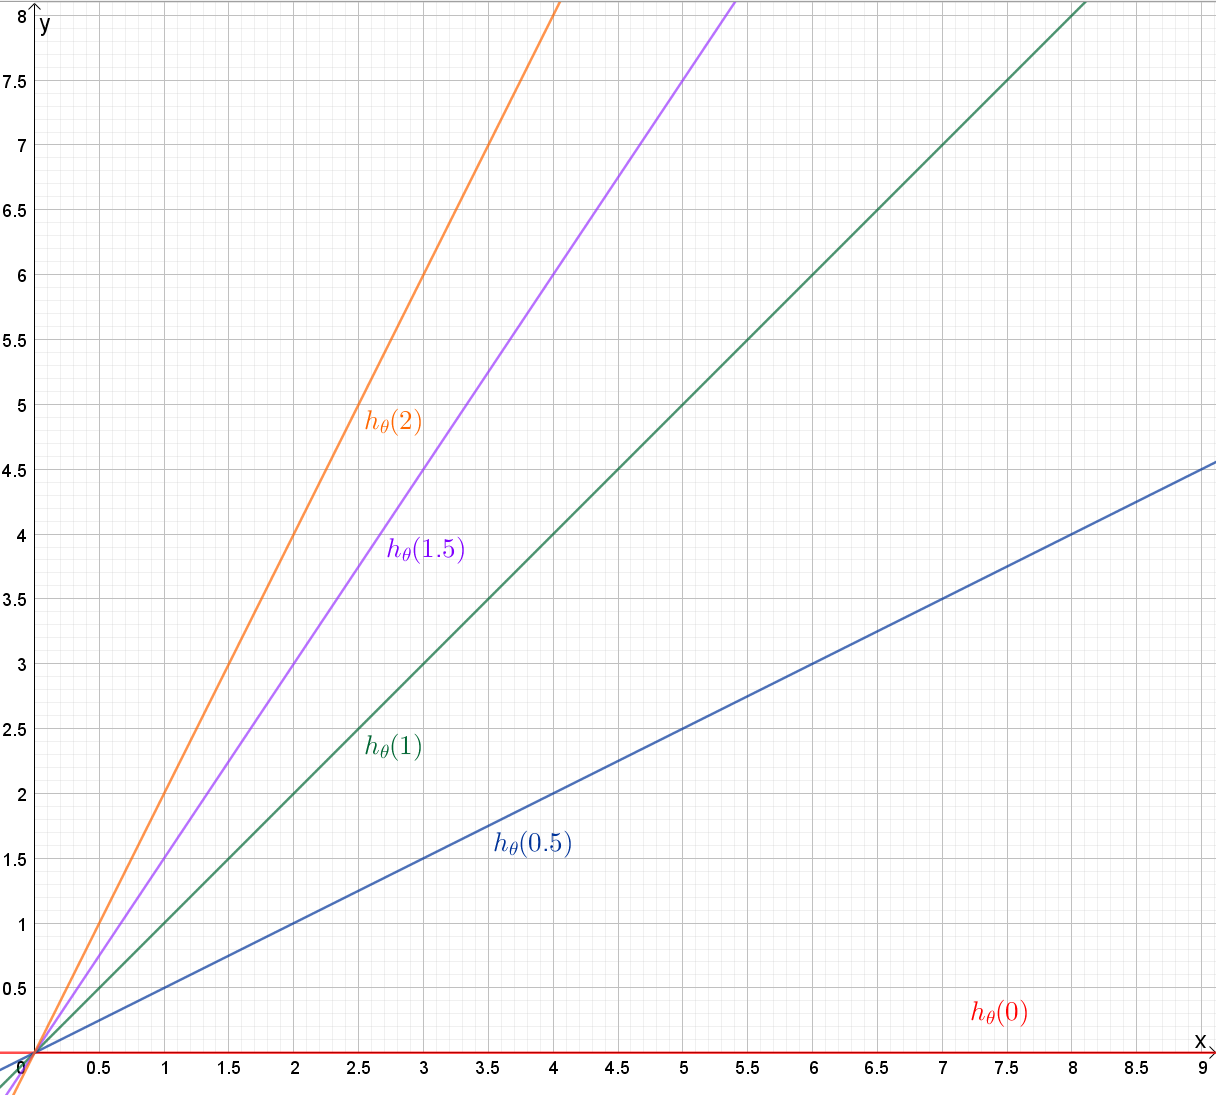
\includegraphics[scale=.5]{Abbildungen/Lineare_Regression_3}}
%\subfigure[f($\theta_{1}$)]{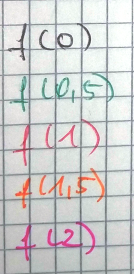
\includegraphics[scale=.5]{Abbildungen/Lineare_Regression/Gradientenabstiegsverfahren3}}
\subfigure[J($\theta_{1}$)]{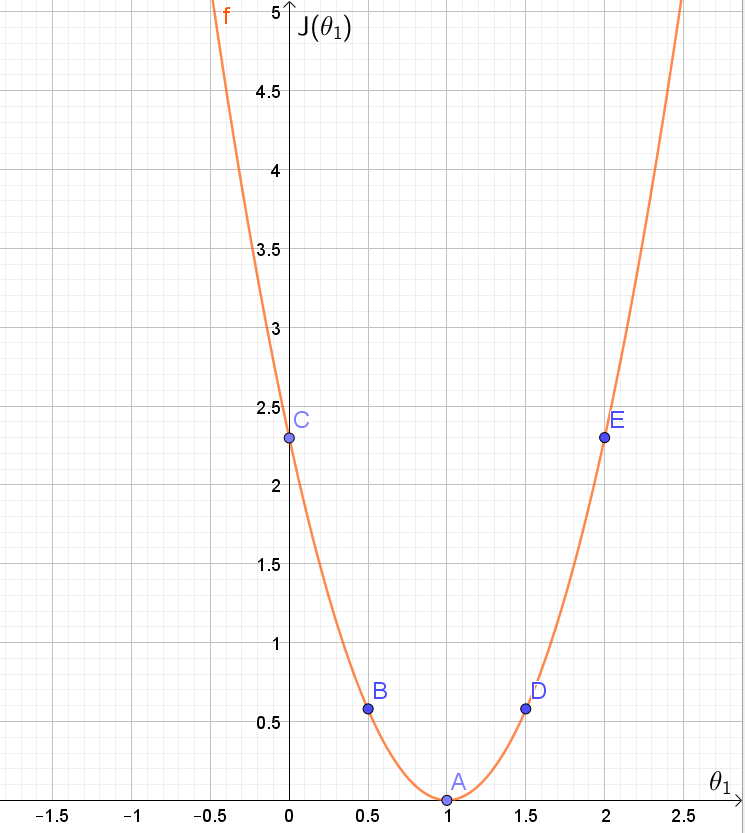
\includegraphics[scale=.5]{Abbildungen/Lineare_Regression_4}}
\label{Intuition Kostenfunktion}
\caption{Intuition Kostenfunktion}
\end{figure}
\\\\
Die Ableitung $J'(\theta_{1})=0$ gilt für $\theta_{1}=1$, was in diesem Beispiel exakt dem Minimum der Funktion entspricht. Wird der Parameter $\theta_{0}$ hinzugezogen, ergibt sich statt einer Parabel eine konvexe Funktion.\\\\
%
\begin{figure}[htbp]
\centering
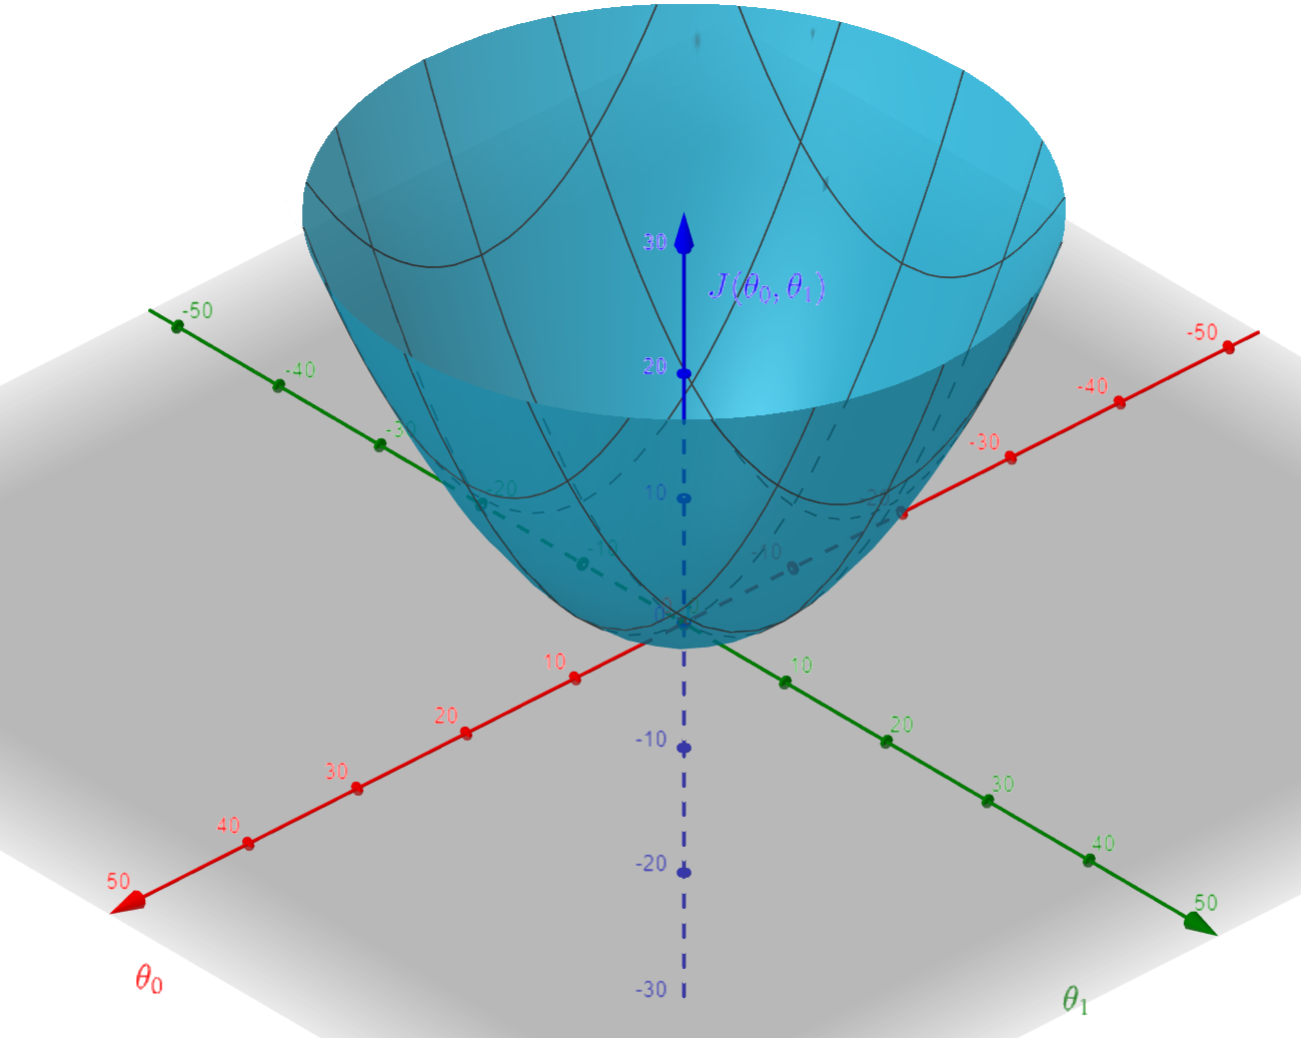
\includegraphics[scale=.5]{Abbildungen/Lineare_Regression_5}
\label{Konvexe Funktion}
\caption{Beispiel konvexe Funktion}
\end{figure}\\
\\\\
Auch diese hat ein globales Minimum. Demnach ist die Kostenfunktion nach  $\theta_{0}$ und $\theta_{1}$ partiell zu differenzieren, um das Minimum zu berechnen. Dafür wird die Kostenfunktion um die Konstante 2 erweitert, was die Berechnung der Ableitung erleichtert.\\\\
$J (\theta_{0},\theta_{1})=\frac{1}{2*n}\sum_{i=1}^{n} (y_i-(\theta_{0}+\theta_{1}*x_i))^{2}$\\\\
Demzufolge ergeben sich folgende innere Ableitungen für $h_{\theta}(x_i)$ nach jeweils $\theta_{0}$ und $\theta_{1}$:\\\\
$h_{\theta}(x_i)=\theta_{0}+\theta_{1}*x_i$\\\\
$J (\theta_{0},\theta_{1})= \frac{1}{2*n}\sum_{i=1}^{n} (y_i-(\theta_{0}+\theta_{1}*x_i))^{2}$\\\\
$\frac{\delta}{\delta \theta_{0}} h_{\theta} (x_i)= \frac{\delta}{\delta \theta_{0}} (\theta_{0}+\theta_{1}*x_i)=\frac{\delta}{\delta \theta_{0}} \theta_{0}+\frac{\delta}{\delta \theta_{0}} \theta_{1}*x_i=1+0=1$\\\\
$\frac{\delta}{\delta \theta_{1}} h_{\theta} (x_i)= \frac{\delta}{\delta \theta_{1}} (\theta_{0}+\theta_{1}*x_i)=\frac{\delta}{\delta \theta_{1}}+\theta_{0}+\frac{\delta}{\delta \theta_{1}} \theta_{1}x_i=0+x_i =x_i$\\\\
\\\\
Die äußere Ableitung ist:\\\\
$J`_{\theta_{0},\theta_{1}} (x_i)=\frac{1}{2*n}\sum_{i=1}^{n} 2 (h_{\theta}(x_i)-y_i)= \frac{1}{n}\sum_{i=1}^{n}  (h_{\theta}(x_i)-y_i)$\\\\
Die partielle Ableitung von $J (\theta_{0},\theta_{1})$ ergibt nach der Kettenregel für $\theta_{0}$ und $\theta_{1}$ folgende Terme:\\\\
$\frac{\delta}{\delta \theta_{0}} J(\theta_{0},\theta_{1})= \frac{1}{n}\sum_{i=1}^{n} (h_{\theta} (x_i)-y_i)$\\\\
$\frac{\delta}{\delta \theta_{1}} J(\theta_{0},\theta_{1})= \frac{1}{n}\sum_{i=1}^{n} (h_{\theta} (x_i)-y_i)*x_i$\\\\
% Bild Anstieg $a$ und $b$ Richtung neuer Wert
Nachdem die Grundlagen des Verfahrens beschrieben sind, sind die einzelnen Berechnungen zu einem Algorithmus zusammenzufassen. Zunächst werden für die Parameter $\theta_{0}$ und $\theta_{1}$ zufällige Werte gewählt. Dann wird für alle $x_i$-Werte die Fehlerfunktion ausgerechnet. Die Anstiege von $\theta_{0}$ und $\theta_{1}$ geben per Vorzeichen die Richtung an, in welcher der Folgewert für $\theta_{0}$ und $\theta_{1}$ gewählt wird. Das Ziel ist, das globale Minimum der Fehlerfunktion zu ermitteln. Dazu muss ein Konvergenzkriterium bestimmt werden. Das Konvergenzkriterium kann verschieden definiert werden. In vielen Fällen wird der Algorithmus über eine vorgegebene Anzahl von Iterationen ausgeführt. Andere Algorithmen vergleichen die Änderungen der Werte der Fehlerfunktion und brechen bei Unterschreiten eines vorgegebenen Mindestdeltas ab. Die Größe der Änderung pro Iteration wird durch einen Hyperparameter, der Lernrate $\alpha$, bestimmt. Die Zuweisung der neuen Werte wird durch das Zeichen $:=$ dargestellt. Daraus folgt:\\\\
$\theta_{0}:= \theta_{0} - \alpha * \frac{\delta}{\delta \theta_{0}} J(\theta_{0},\theta_{1})$\\\\
$\theta_{1}:= \theta_{1} - \alpha * \frac{\delta}{\delta \theta_{1}} J(\theta_{0},\theta_{1})$\\\\
Das Gradient-Descent Verfahren ist ein allgemeines Konzept, das in vielen Bereichen Anwendung findet. Je nach Anwendung kann auch das Gradient-Descent Verfahren optimiert werden. Für stabile Funktionen und wenige Testdaten, wie in diesem Beispiel, ist das \textbf{Batch-Gradient-Descent} Verfahren geeignet.\newpage
Dabei wird die Summe der Fehlerfunktion über alle Testdatensätze berechnet und eine stabiler Wert führt zum Update und damit zu einer stabilen Konvergenz des Abstiegs.
\footnote{Andrew Ng- YouTube Video- 2.4-Linear Regression With One Variable | Cost Function Intuition 2}
\footnote{Andrew Ng- YouTube Video- 2.5-Linear Regression With One Variable | Gradient Descent}
\footnote{Andrew Ng- YouTube Video- 2.6-Linear Regression With One Variable | Gradient Descent Intuition}
\\\\
Das \textbf{Stochastic-Gradient-Descent} Verfahren führt ein Update der Parameter nach jedem einzelnen Datensatz durch. Abhängig von der Anwendung kann dies schneller zur Konvergenz führen. In vielen Fällen kann es aber dazu führen, das die Fehlerfunktion stark variiert und nicht mehr konvergiert. Dieses Verfahren benötigt einen höheren Rechenaufwand als das vorgenannte.\\\\
In vielen Anwendungen wird eine Kombination aus den beiden beschriebenen Verfahren, das \textbf{Mini-Batch-Gradient-Descent} Verfahren gebildet. Dabei wird das Stochastic-Gradient-Descent Verfahren auf kleinere Mengen des Datensatze den Minibatches, z.B. auf 256 Datensätze gleichzeitig, angewendet. Die Vorteile der beiden Verfahren werden somit kombiniert.
\footnote{Andrew Ng- YouTube Video-Lecture 17.2 — Large Scale Machine Learning | Stochastic Gradient Descent}
\\\\
\textbf{Umsetzung im Python Code}\\\\
%
Für die erste Implementierung eines Maschine Learning Algorithmus wurde die Vorhersage von Wohnungspreisen anhand der Quadratmeterzahl gewählt. Ein linearer Zusammenhang zwischen Wohnfläche und Preis ist allgemein bekannt. Im ersten Beispiel wurde die Bibliothek SciKit-Learn verwendet. Die Abbildungen 3.5 und 3.6 zeigen in Google CoLab das Laden der Daten aus einer CSV Datei aus dem Github Repository. Danach werden die Daten trainiert und die berechneten Parameter inklusive einem Diagramm der Datenwerte und der Regressionsgeraden ausgegeben.\newpage
Die zweite Variante ist eine Implementierung analog zu den vorgestellten Formeln. Die Daten werden wieder geladen und anschließend skaliert. Dieser Prozess ist auf Grund der unterschiedlichen Größenordnungen zur Berechnung notwendig. Im obigen Programm übernimmt diese Aufgaben die Bibliotheksfunktion. Die Implementierung gibt ein ganz ähnliches Diagramm wie die Bibliotheksimplementierung aus.
\footnote{Jannis Seemann- Udemy Kurs Machine Learning von A-Z - Section 5- Python: Lineare Regression Teil 1}
\footnote{Jannis Seemann- Udemy Kurs Machine Learning von A-Z - Section 5- Python: Lineare Regression Teil 2}
\newline
%
\begin{figure}[hp]
\centering
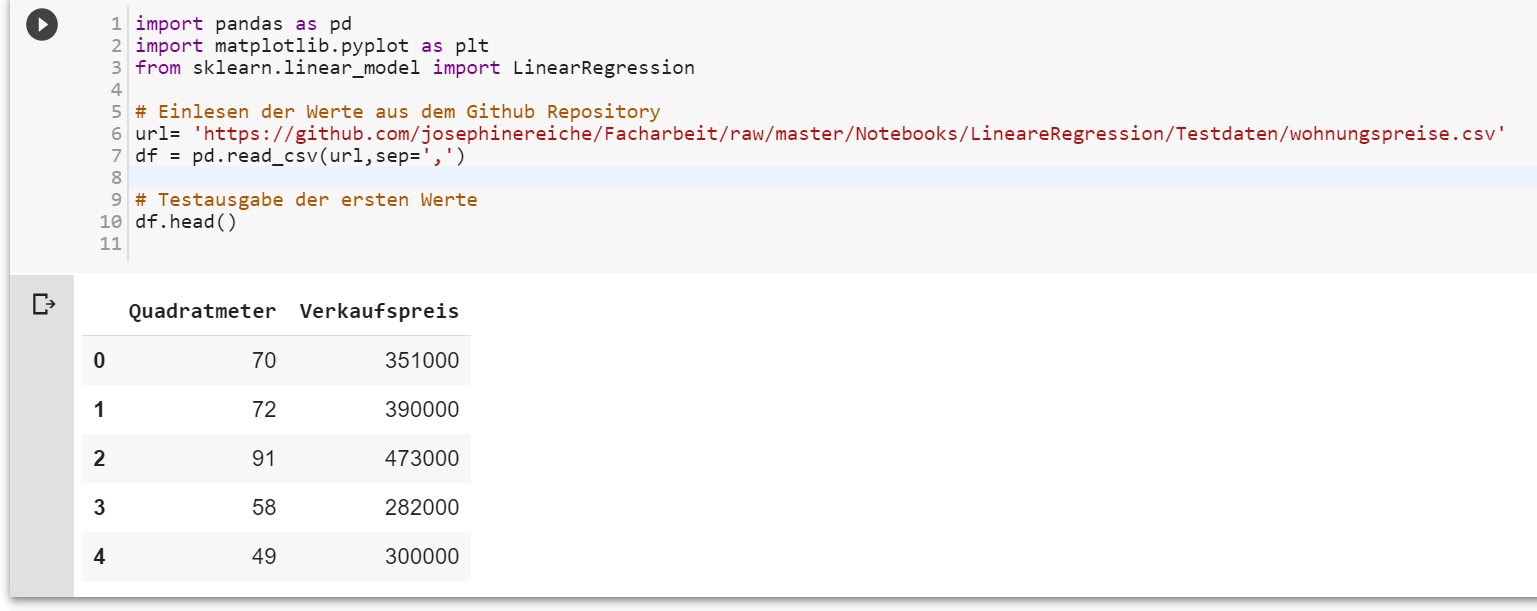
\includegraphics[scale=.75]{Abbildungen/Lineare_Regression_Python_1}
\label{Konvexe Funktion}
\caption{Laden der Daten und Module}
\end{figure}\\
%
\begin{figure}[hp]
\centering
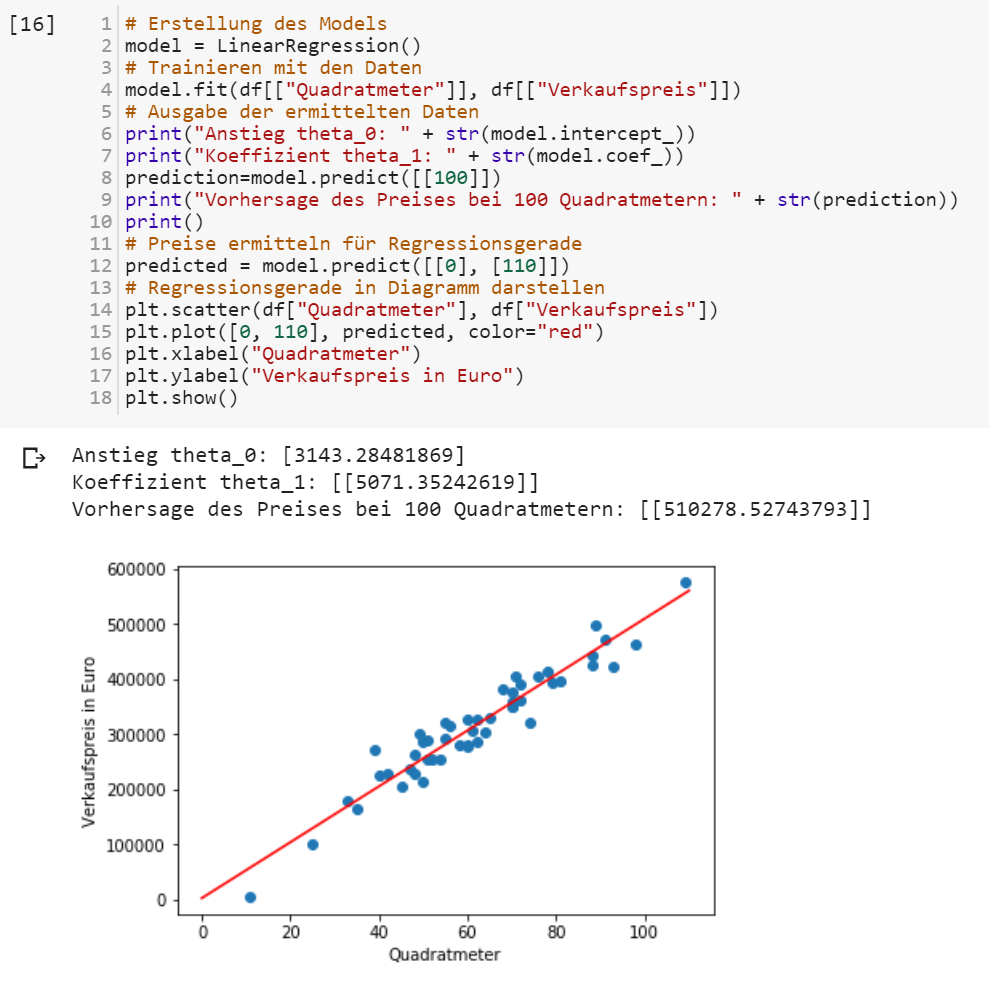
\includegraphics[scale=.75]{Abbildungen/Lineare_Regression_Python_2}
\label{Konvexe Funktion}
\caption{Programmcode und Ausgabe}
\end{figure}\\
%
\begin{figure}[hp]
\centering
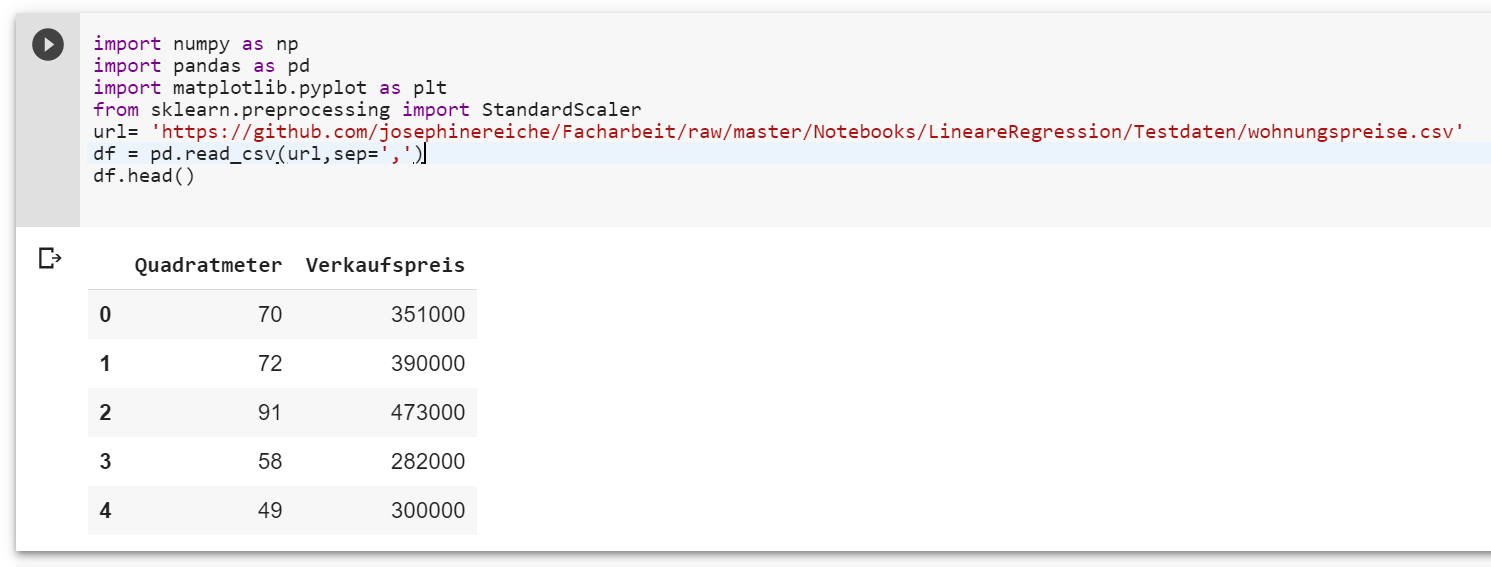
\includegraphics[scale=.75]{Abbildungen/Lineare_Regression_Python_3}
\label{Konvexe Funktion}
\caption{Laden der Daten und Module}
\end{figure}\\
%
\begin{figure}[hp]
\centering
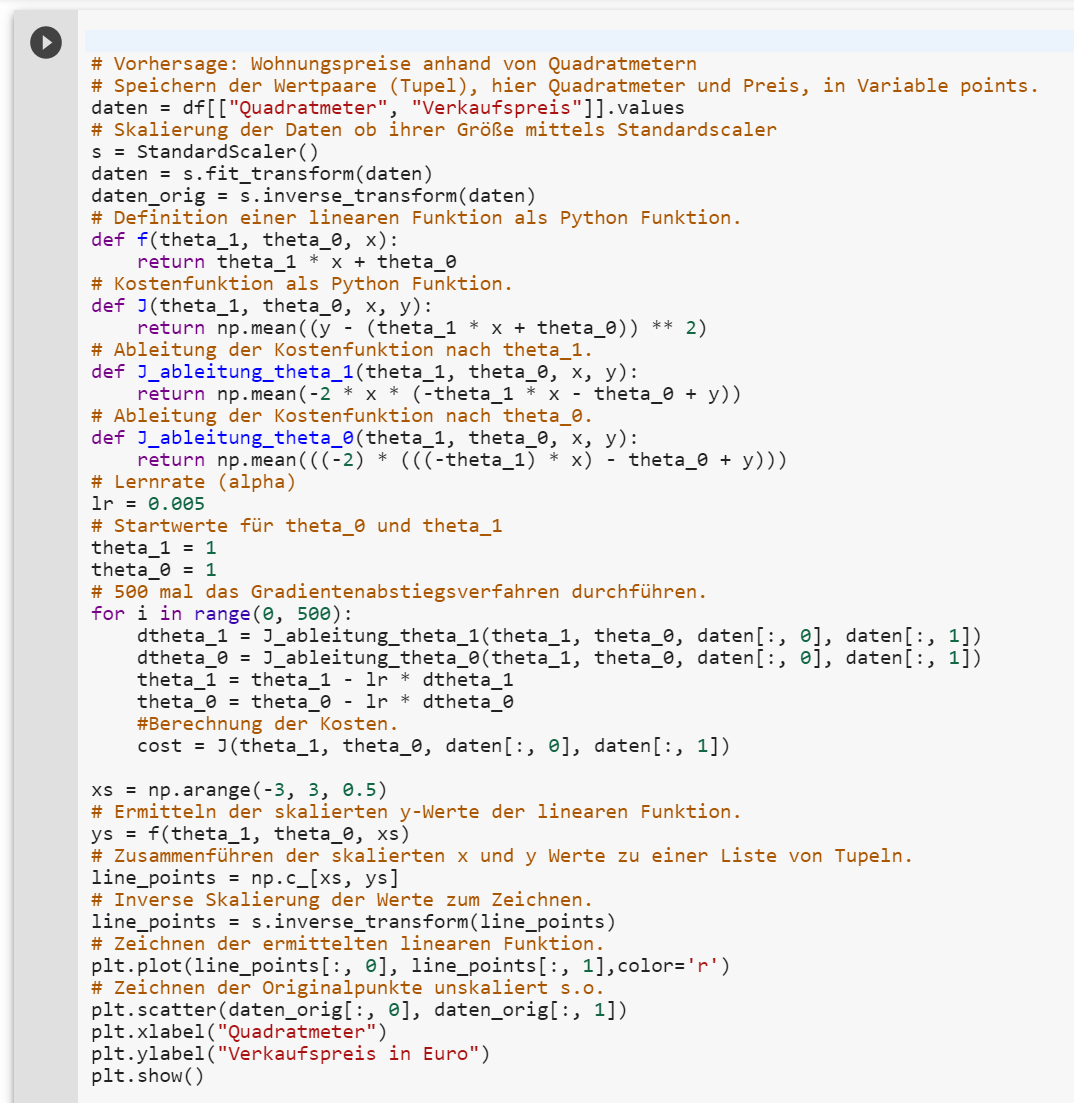
\includegraphics[scale=.75]{Abbildungen/Lineare_Regression_Python_4}
\label{Konvexe Funktion}
\caption{Implementierung}
\end{figure}\\
%
\begin{figure}[hp]
\centering
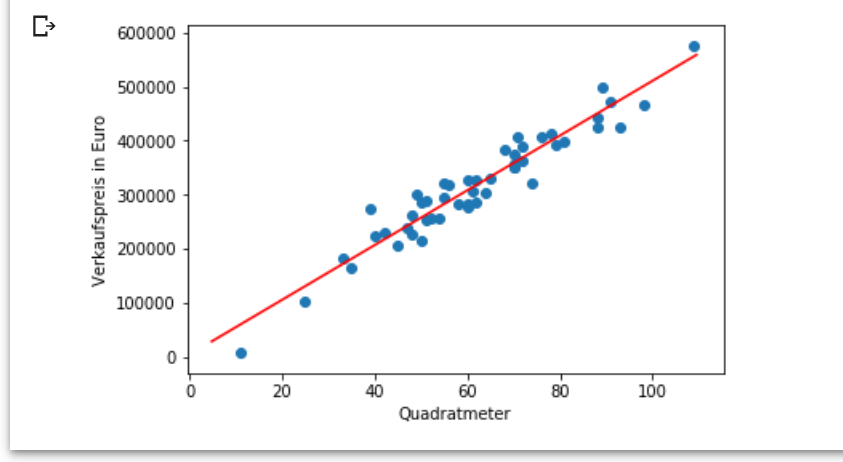
\includegraphics[scale=.75]{Abbildungen/Lineare_Regression_Python_5}
\label{Konvexe Funktion}
\caption{Ausgaben}
\end{figure}
\newpage
\subsection{Multiple Lineare Regression}
Die multiple lineare Regression ist ein statistisches Verfahren und dient der Verallgemeinerung der einfachen linearen Regression. Ziel ist es, die Beziehung zwischen zwei oder mehreren Variablen durch Anpassen einer linearen Gleichung an die beobachteten Daten zu modellieren. Jedem Wert der unabhängigen Variablen ${x}$ ist ein Wert der abhängigen Variablen ${y}$ zugeordnet.\\\\
Die bisherige Formel für die lineare Regression: $h_{\theta}(x)=\theta_{0}+\theta_{1}*x$ wird zu $h_{\theta}(x)=\theta_{0}+\theta_{1}*x_{1}+\theta_{2}*x_{2}+...+\theta_{n}*x_{n}$ erweitert. Zum besseren Handling der Vektoren und Matrizen ist es sinnvoll $x_{0}=1$ und somit $h_{\theta}(x)=\theta_{0}*x_{0}+\theta_{1}*x_{1}+\theta_{2}*x_{2}+...+\theta_{n}*x_{n}$ mit
${x}=\left(\begin{array}{c} x_{0} \\\ x_{1} \\\ x_{2} \\\ ... \\\ x_{n}  \end{array}\right) {\in \rm I\!R^{n+1}}$ und  
%${R^{n+1}}$\\\\
${\Theta}=\left(\begin{array}{c}\theta_{0} \\\ \theta_{1} \\\ \theta{2} \\\ ... \\\ \theta_{n}  \end{array}\right) {\in \rm I\!R^{n+1}}$ also ${\theta^{T}x}$ zu erhalten.\\\\
Nun kann die oben aufgestellte Kostenfunktion wie folgt verallgemeinert werden, wobei ${i}$ den Datensatzindex, ${j}$ den Variablenindex und ${m}$ die Anzahl der Datensätze bezeichnet:
\footnote{Andrew Ng- YouTube Video- Lecturev4.1 — Linear Regression With Multiple Variables - (Multiple Features)}
\footnote{Jannis Seemann- Udemy Kurs Machine Learning von A-Z - Section 8- Intuition: Lineare regression mit mehren Variablen Teil 1}
\footnote{Jannis Seemann- Udemy Kurs Machine Learning von A-Z - Section 8- Intuition: Lineare regression mit mehren Variablen Teil 2}
\\\\
$J (\Theta_{j})= \frac{1}{2*m}\sum_{i=1}^{m} (h_{\theta}(x_{i})-y_{i})^{2}$\\\\
Die Minimierung der Kostenfunktion erfolgt dank der Ableitungsregeln algorithmisch vorteilhaft durch:\\\\
$\frac{\delta}{\delta \Theta_{j}} J(\Theta_{\theta_{0}, \theta_{1}..\theta_{n+1}})= \frac{\delta}{\delta \Theta_{j}} J(\Theta_{j})=\frac{1}{m}\sum_{i=1}^{m} (h_{\theta} (x_{j,i})-y_{i,j})*x_{i,j}$\\\\
Entsprechend gilt für die Update-Regel des Gradient-Descent Verfahren:\\
$\theta_{j}:= \theta_{j} - \alpha * \frac{\delta}{\delta \Theta_{j}} J(\Theta_{j})$\\\\
%TODO Endformulierung???
\end{enumerate}
%Logistische Regression
\par\bigskip
\section{Logistische Regression}
In der Praxis des Machine-Learning haben Klassifikationsprobleme eine noch größere Bedeutung als die Vorhersage von diskreten Werten. Das Verfahren der logistischen Regression wird, je nach Anwendung, in eine dieser Kategorien eingeteilt:\\
\begin{enumerate}
\item [a)]
Die binäre logistische Regression bildet die Eingaben verschiedener Variablen auf nur zwei Elemente einer Menge ab z.B. ${0,1}$. Diese Art der Regression hilft dem Nutzer Ja/Nein Fragen zu entscheiden. Zum Beispiel ist eine E-Mail Spam? Ist ein Tumor bösartig? Wird ein Nutzer einen Vertrag erfüllen?
\item [b)]
Die multinominale logistische Regression ermöglicht eine Einordnung der Ergebnisse in mehr als zwei verschiedene Kategorien. So könnte etwa das Abstimmverhalten von Wählern nach Parteien ermittelt werden.
\item [c)]
Die ordinale logistische Regression, kategorisiert nach geordneten Kategorien, z.B. der Einteilung von Hotels nach Sternen (1-5).
\end{enumerate}
Im folgenden wird nur der Fall a) betrachtet, da die binäre Regression den grundlegenden Aufbau der logistischen Regression sehr gut illustriert. Allgemein ist die Logistische Regression ein statistisches Verfahren, mit dem der Wert Y in Abhängigkeit von einer oder mehreren unabhängigen Variablen X geschätzt wird. Im Unterschied zur linearen Regression setzt die binäre logistische Regression für den Ergebniswert Y entweder den Wert 1 oder den Wert 0 an. In der Literatur wird bei einer binären Fragestellung der Wert 1 meist einer positiven Fallentscheidung und der Wert 0 einer negativen Fallentscheidung zugeordnet. Die Vorgabe, dass die Ergebnismenge der logistischen Hypothesefunktion auf einer binären Menge abgebildet werden allein, schließt eine Anwendung der linearen Regression nicht von vornherein aus. Die folgende Abbildung der kreisförmig angeordneten binären Werte legt aber intuitiv den Schluss nahe, dass reine lineare Funktionen nicht für diese Problemkategorie geeignet sind. Welche Funktion erfüllt dann die notwendigen Voraussetzungen?
\footnote{Andrew Ng- YouTube Video- Lecture 6.1 — Logistic Regression | Classification}
\par\bigskip
\\\\\
\\\\\
\subsubsection{Sigmoidfunktion}
Gesucht ist eine Funktion $0 \leq h_{\theta}(x)=\Theta^Tx \leq 1$. Eine solche Funktion ist die Sigmoid-Funktion $g(z)=\frac{1}{1+e^{-z}}$ mit $x \in \rm I\!R$ und $g(z) \in \{0,1\}$. Diese wird auch die logistische Funktion genannt. Es existieren auch andere Funktionen mit den gesuchten Eigenschaften, die Sigmoidfunktion ist aber für die noch folgenden Operationen besonders gut geeignet. Die Abildung zeigt den Verlauf der Sigmoidfunktion, die für $x=0$ bei 0,5 liegt und sich im negativen Unendlichen der 0 und im positiv Unendlichen der 1 annähert.\\
%
\begin{figure}[h]
\centering
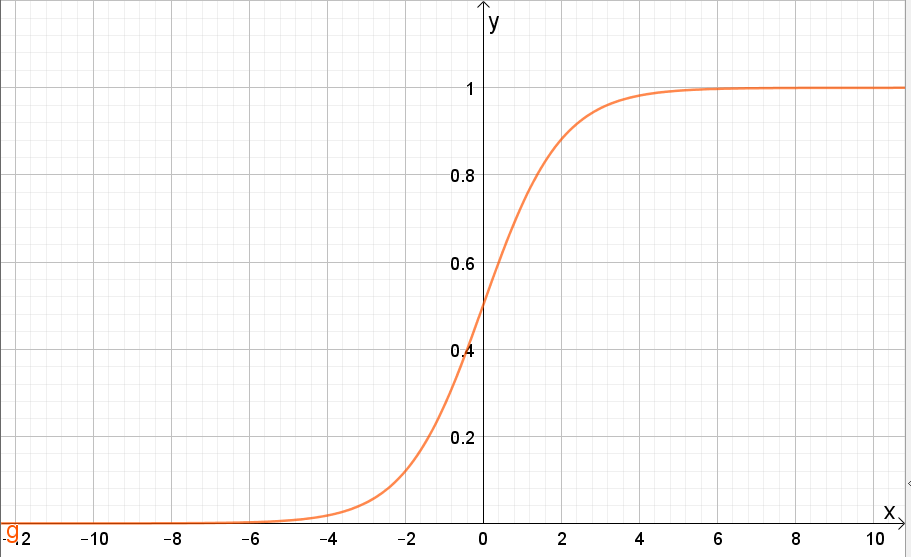
\includegraphics[scale=.74]{Abbildungen/Logistische_Regression_1}
\caption{Abb: Sigmoid Funktion}
\label{figure}
\end{figure}
\\\\
Setzt man nun $h_\theta(x)=g(\Theta^Tx)$ erhält man als Hypothesefunktion $h_{\theta}(x)=\frac{1}{1+e^{-\Theta^Tx}}$.\\ 
Die Ausgabewerte der Funktion werden als Wahrscheinlichkeiten für die binäre Wertemenge $\{0,1\}$ interpretiert. Anders formuliert ist $h_{\theta}(x)$ die geschätzte Wahrscheinlichkeit für $y=1$ für einen Eingabewert $x$. Ist zum Beispiel für einen ermittelten SPAM-Wert $x$ $h_{\theta}(x)=0.75$, dann ist die E-Mail zu 75\% SPAM, da die Wahrscheinlichkeit für $y=1$ bei 0.75 liegt. Die einzelnen Eingabewerte $x$ werden, wie bei der linearen Regression, mit jeweils einem $\theta$ parametrisiert, so dass die Wahrscheinlichkeit $y=1$ auch als $h_{\theta}(x)=P(y=1|x;\theta)$ notiert werden kann. Weiterhin gelten natürlich die innerhalb der Wahrscheinlichkeitsrechnung allgemein geltenden Bedingungen $P(y=0\mid x;\theta)+ P(y=1)\mid x;\theta)=1$ entsprechend $1-P(y=0\mid x;\theta)=P(y=1)\mid x;\theta)$.
\footnote{Andrew Ng- YouTube Video- Lecture 6.1 — Logistic Regression |Hypothesis Representation}
\footnote{Jannis Seemann- Udemy Kurs Machine learning A-Z- Section 21- Intuition: Logistische Regression}
\par\bigskip
\\\\
\\\\
\subsection{Entscheidungsgrenzen}
Die Entscheidungsgrenze (engl. decision-boundary) ist für die Ermittlung der Wahrscheinlichkeiten der Ausgangswerte entscheidend und durch die Hypothesefunktion definiert. Für die Sigmoidfunktion gilt $y=1$ wenn $h_{\theta}(x)=g(\Theta^Tx) \geq 0.5$ und analog $y=0$ wenn $h_{\theta}(x)=g(\Theta^Tx) < 0.5$. Bei der Sigmoidfunktion $g(z)=g(\Theta^Tx)$ trifft dies für $\Theta^Tx \geq 0$ bzw. $\Theta^Tx < 0$ zu. Folgende Beispiele helfen die Berechnung und Intuition der Entscheidungsgrenzen zu verdeutlichen.\\
%
\begin{figure}[h]
\centering
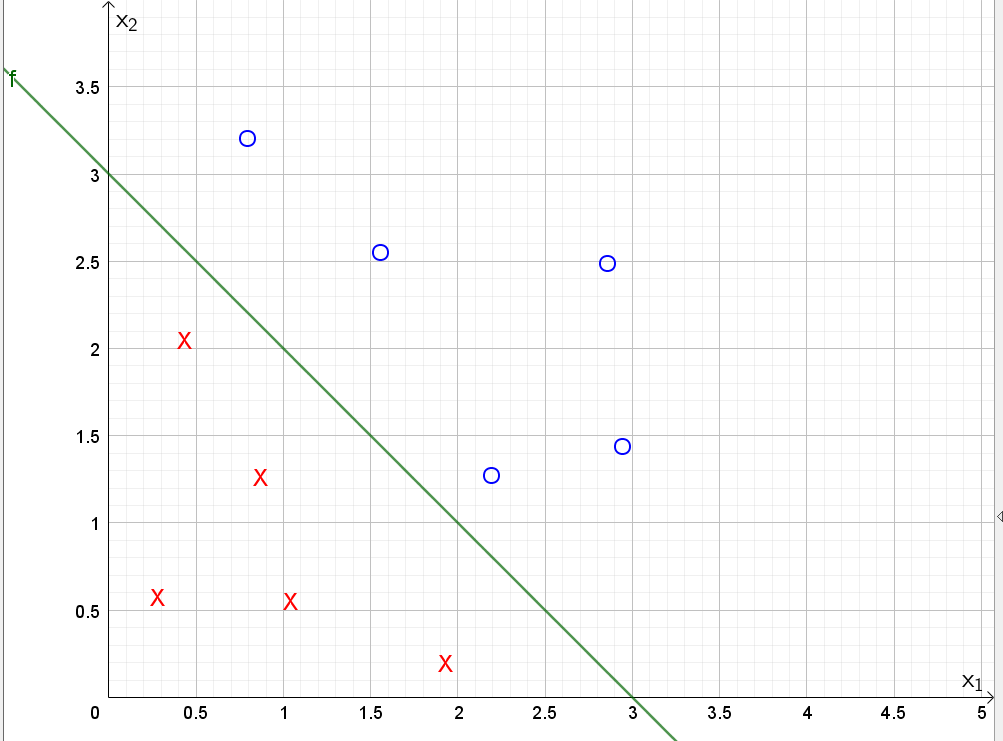
\includegraphics[scale=.74]{Abbildungen/Logistische_Regression_2}
\caption{Beispiel einer Linearen Entscheidungsgrenze}
\label{figure}
\end{figure}
\\
Gegeben ist eine Funktion $h_\theta(x)=g(\theta_{0}+\theta_{1}x_{1}+\theta_{2}x_{2})$ mit $\Theta=\{-3,1,1\}$, dann ist $y=1$, wenn $h_\theta(x) \geq 0.5$ und $\Theta^Tx \geq 0$ also $-3+x_{1}+x_{2} \geq 0$ bzw. $x_{1}+x_{2} \geq 3$. Für $y=0$ gilt letztlich analog $x_{1}+x_{2} < 3$. Die Grafik in der Abbildung verdeutlicht den Verlauf der Entscheidungsgrenze. Funktionen, die eine Entscheidungsgrenze abbilden sind in der Regel komplexer und wie eingangs behauptet selten linear. Ein beherrschbares Beispiel sei mit $h_\theta(x)=g(\theta_{0}+\theta_{1}x_{1}+\theta_{2}x_{2}+\theta_{3}x_{1}^2+\theta_{4}x_{2}^2), \Theta=\{-1,0,0,1,1\}$ gegeben. Werden die Werte entsprechend eingesetzt, gilt $y=1$, wenn $x_{1}^2+x_{2}^2 \geq 1$. Die Abbildung illustriert folgend die beschriebenen Parabeln als Entscheidungsgrenze.
\footnote{Andrew Ng- YouTube Video- Lecture 6.3 — Logistic Regression | Decision Boundary}
\\
%TODO Mengen in der Grafik zu x=1 und x=0 zuordnen
%
\begin{figure}[h]
\centering
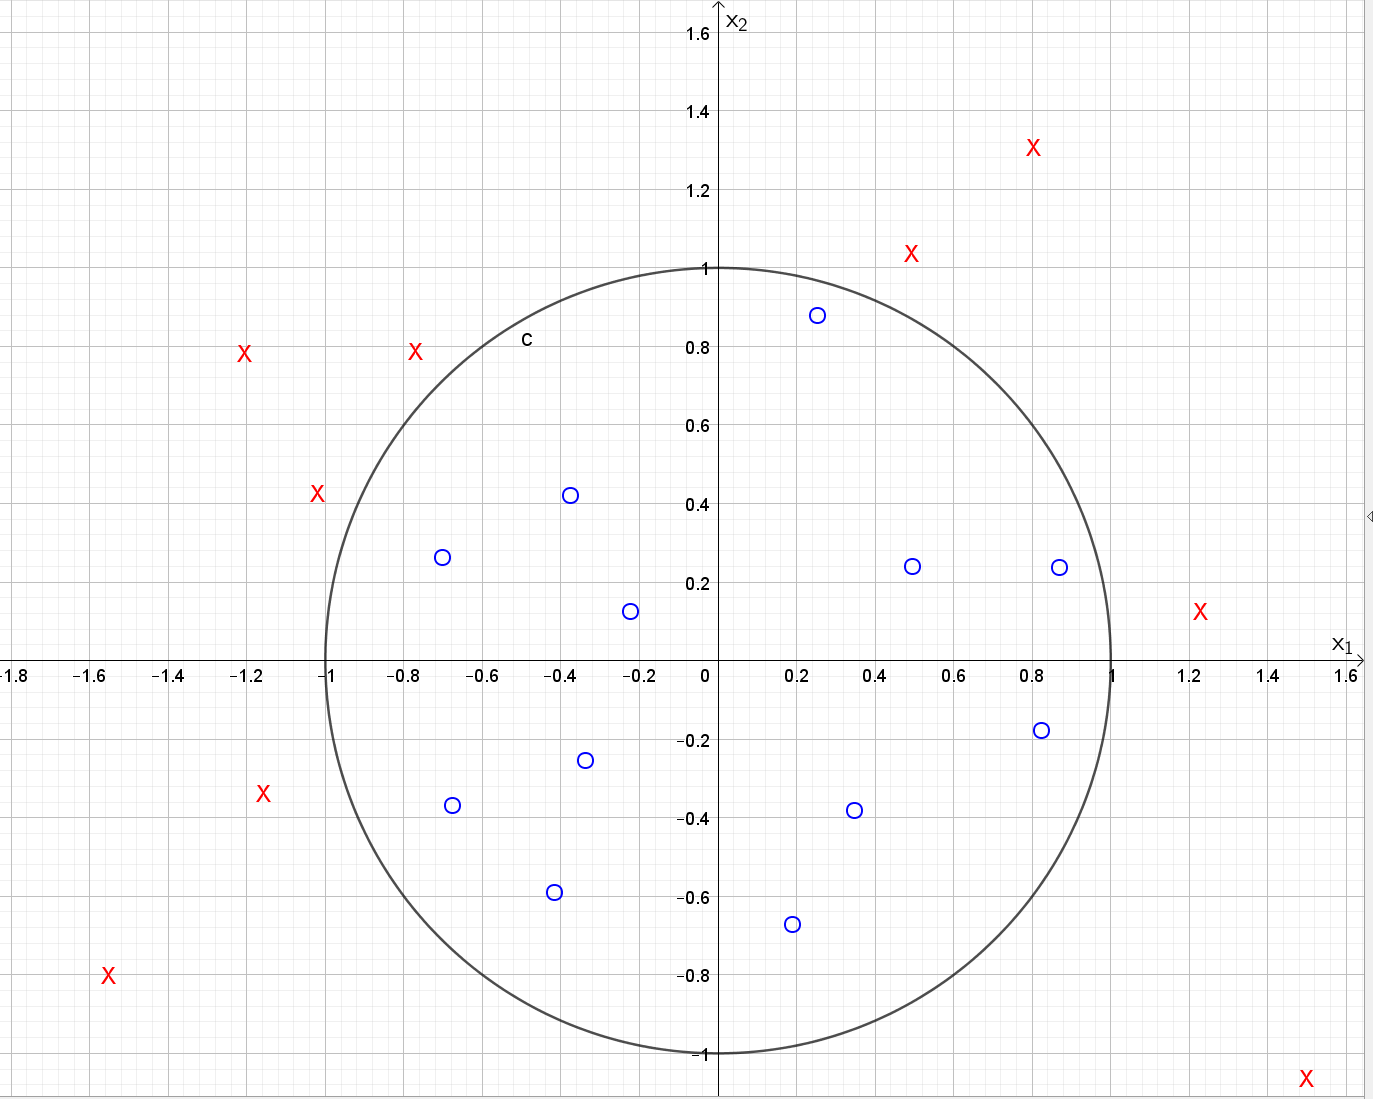
\includegraphics[scale=.74]{Abbildungen/Logistische_Regression_3}
\caption{Beispiel einer nichtlinearen Entscheidungsgrenze}
\label{figure}
\end{figure}
\\
Wie werden die hier vorgegebenen Werte für $\Theta$ ermittelt?\newpage
\subsection{Kostenfunktion}
Auch für die logistische Regression wird eine Kostenfunktion $J(\Theta)$ hergeleitet, die mit dem bereits bekannten Gradientenabstiegsverfahren minimiert werden soll. Zunächst scheint es möglich, die schon im Kapitel 3.1.2 eingeführte Kostenfunktion
\\\\
$J(\Theta)=\frac{1}{m}\sum\limits_{i=1}^{m}\frac{1}{2}*(h_{\Theta}x^{(i)}-y^{(i)})^{2}$\\\\zu nutzen. Die Ableitung des Funktionsterms $h_\theta(x)=\frac{1}{1+e^{-\Theta^Tx}}$ ist nicht konvex, das heißt es gibt mehrere lokale Minima. Das optimale also globale Minimum ist mit dem Gradientabstiegsverfahren so nicht mehr zuverlässig auffindbar. Die Lösung für die Kostenfunktion der logistischen Regression ist durch die Eigenschaften der Logarithmusfunktion gegeben. Zunächst wird der Term innerhalb der Summe durch eine allgemeingültige Kostenfunktion ersetzt, die vom Werten der Hypothesefunktion und dem bekannten Wert für y abhängt. Zur besseren Darstellung wird auf die Indizes der Daten x und y verzichtet.\\\\
$J(\Theta)=\frac{1}{m}\sum\limits_{i=1}^{m}Cost(h_{\Theta}(x), y)$\\\\
Ziel der zu findenden Funktion ist, bei Übereinstimmung zwischen $h_{\Theta}(x))$ und $y$ einen geringen Wert zu erhalten und bei gegensätzlichem Ergebnis einen möglichst hohen Wert zu erreichen. Dazu eignet sich im betrachteten Definitionsbereich $\{0,1\}$ die negative Logarithmusfunktion in folgender Konstellation:
\footnote{Andrew Ng- Youtube Video - Lecture 6.4 — Logistic Regression |  Cost Function}
\\\\
$Cost(h_{\Theta}(x),y)=\left \{ \begin{array}{ll} -log(h_{\Theta}(x), & y=1\\ -log(1-h_{\Theta}(x)), & y=0 \end{array} \right.$\\
%$Cost(h_{\Theta}(x),y)= -log(h_{\Theta}(x))$, wenn $y=1$\\\\
%$Cost(h_{\Theta}(x),y)= -log(1-h_{\Theta}(x))$, wenn $y=0$\\
%
\begin{figure}[hpt]
\centering
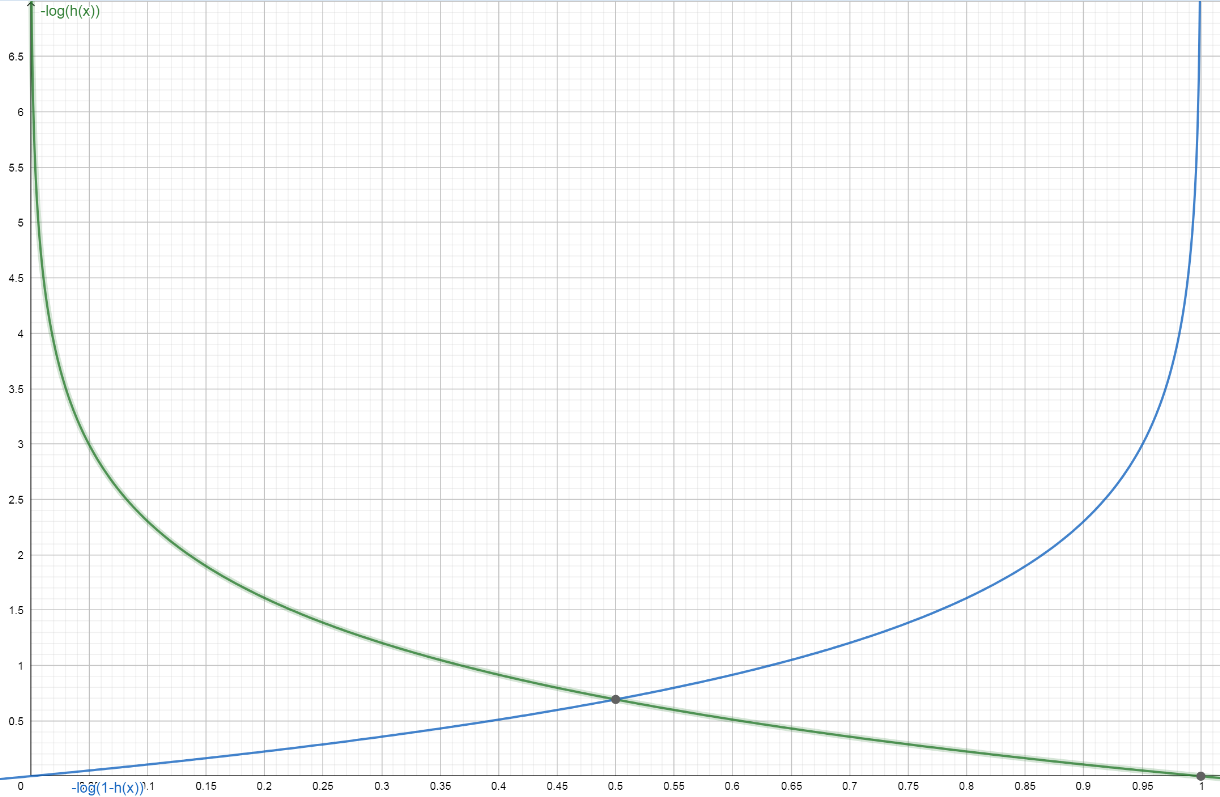
\includegraphics[scale=.44]{Abbildungen/Logistische_Regression_45}
%\subfigure[$y=1$]{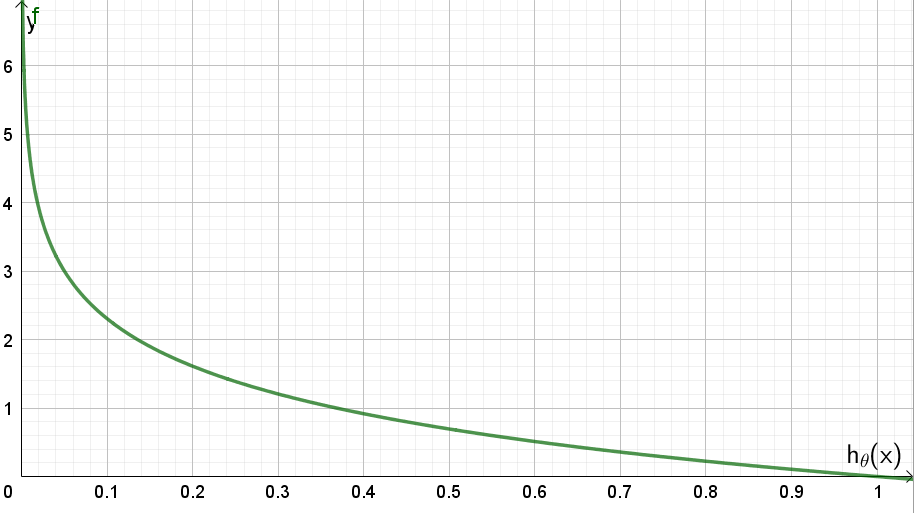
\includegraphics[scale=.75]{Abbildungen/Logistische_Regression_4}}
%\subfigure[$y=0$]{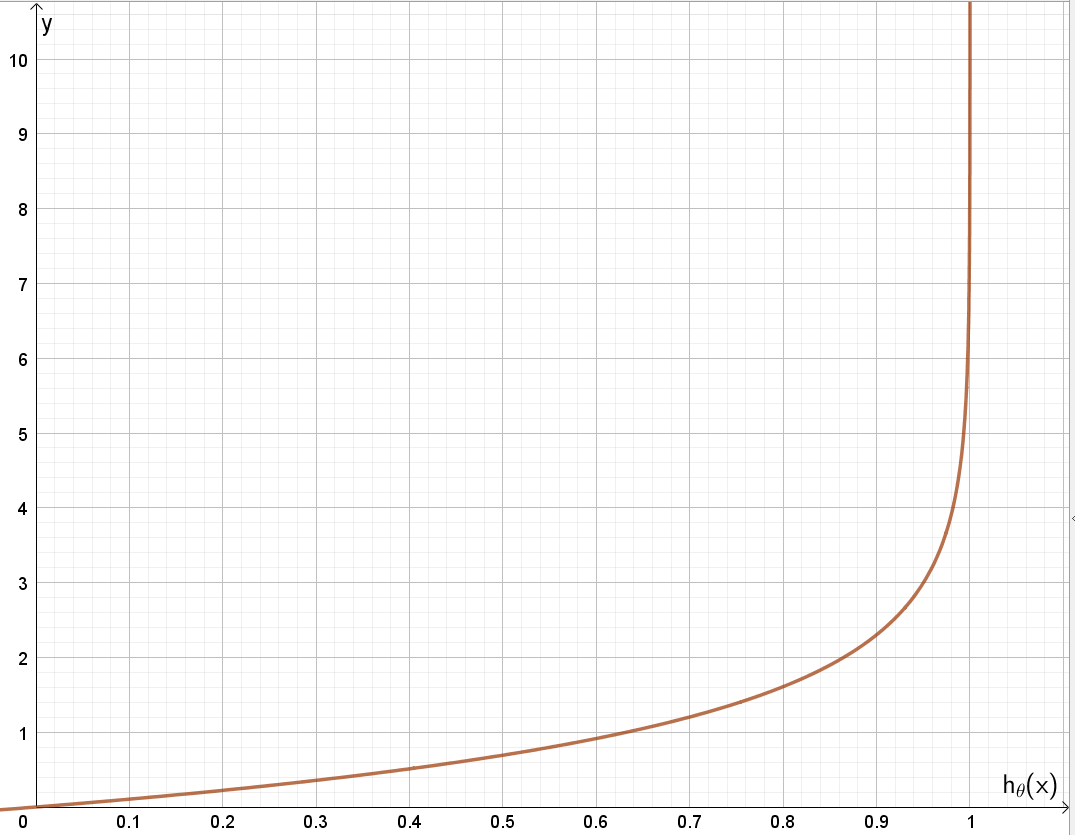
\includegraphics[scale=.75]{Abbildungen/Logistische_Regression_5}}
\caption{Die logistischen Kostenfunktion}
\label{figure}
\end{figure}
\\\\
Die Abbildung 3.8 verdeutlicht die Eigenschaften der logistischen Kostenfunktion grafisch. Für $y=1$ gilt, wenn $h_{\Theta}(x)=1$ dann $Cost=0$ sowie $h_{\Theta}(x)=0$ dann $Cost=\infty$. Für $y=0$ gilt analog, wenn $h_{\Theta}(x)=0$ dann $Cost=0$ sowie $h_{\Theta}(x)=1$ dann $Cost=\infty$. Die Abbildung verdeutlicht die Intuition einer Parabel, die durch die beiden Funktionen entsteht und auch folgende vorteilhafte Berechnungen ermöglicht.
\newpage
Diese beiden Teile der Kostenfunktion lassen sich elegant zusammenfügen:\\\\
$Cost(h_{\Theta}(x),y=-y*log(h_{\Theta}(x))-(1-y)*log(1-h_{\Theta}(x))$\\\\
und in die Ausgangsfunktion einsetzen:\\\\
$J(\Theta)=-\frac{1}{m}[\sum \limits_{i=1}^{m}y^{(i)}*log(h_{\Theta}(x^{(i)})]+(1-y^{(i)})*log(1-h_{\Theta}(x^{(i)})]$\\\\
Der Clou besteht in der Optimierung der Kostenfunktion durch das allgemeingültige Gradientenabstiegsverfahren:\\\\
$\theta_{j}:=\theta_{j}-\alpha*\frac{\delta}{\delta*\theta_{j}}*J(\Theta)$\\\\
dessen partielle Ableitung zu folgendem, bereits aus der linearen Regression bekannten Term führt:\\\\
%$J(\Theta)=-\frac{1}{m}[\sum \limits_{i=1}^{m}y^{(i)}*log(h_{\Theta}(x^{(i)})]+(1-y^{(i)})*log(1-h_{\Theta}(x^{(i)})]$\\
$\theta_{j}:=\theta_{j}-\alpha*\sum\limits_{i=1}^{m}(h_{\Theta}(x^{i})-y^{i})*x_{j}^{i}$\\\\
Bei der algorithmischen Berechnung sind demnach nur die Änderung der Definition von $h_{\Theta}(x)$ und $J(\Theta)$ zu beachten bzw. zu implementieren.
\footnote{Jannis Seemann- Udemy Kurs machine Learning A-Z- Section 21- Intuition: Logistische Regression (Fehlerterm)}
\\\\
\subsection{Logistische Regression in Python}
Die Implementierung der logistischen Regression in Python erfolgt, wie es die o.g. mathematischen Herleitungen beschreiben, ähnlich der linearen Regression. Als Beispiel wurde eine Klassifikation nach Volljährigkeit implementiert. Anhand weniger Daten können passende Wahrscheinlichkeiten zur Volljährigkeit (Alter > 18 y=1) bei $h_{\Theta}(x)\geq0,5$ angegeben werden. Die folgenden Abbildungen dokumentieren den Quellcode und die Resultate bei Ausführung unter Google CoLab.
\footnote{inspiriert nach Jannis Seemann- Udemy Kurs Machine Learning von A-Z- Section 21- logistische regression Python}
\\\\
%
\begin{figure}[hpt]
\centering
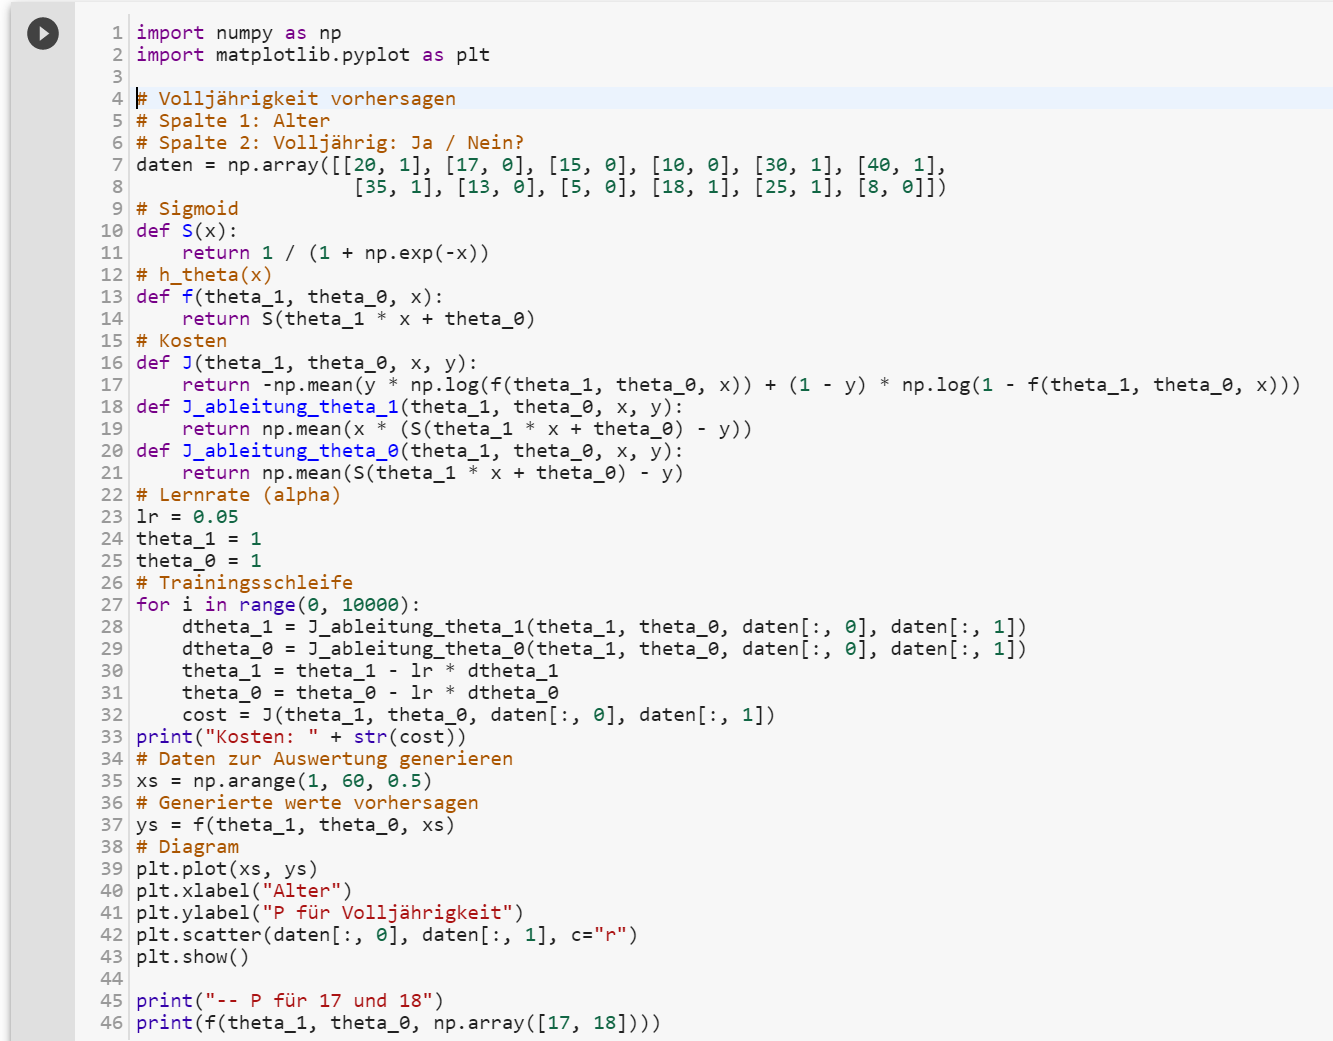
\includegraphics[scale=.84]{Abbildungen/Logistische_Regression_Python_1}
%\subfigure[$y=1$]{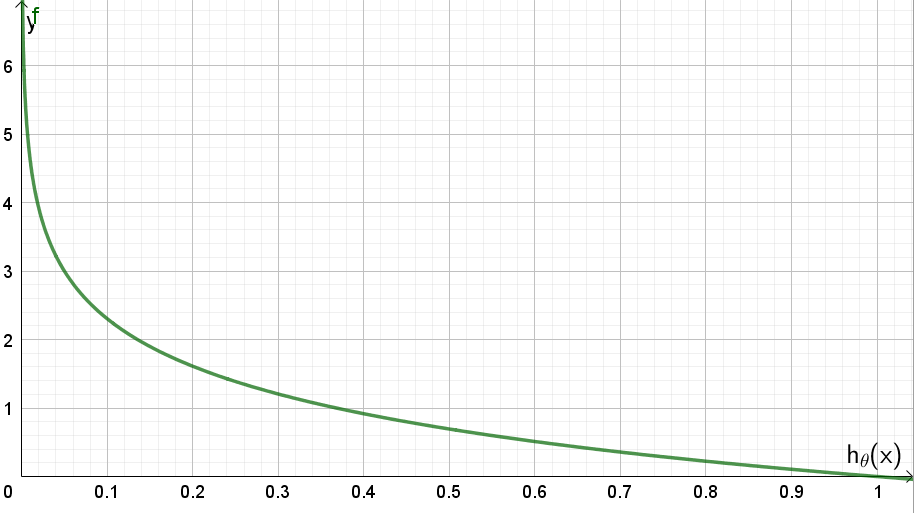
\includegraphics[scale=.75]{Abbildungen/Logistische_Regression_4}}
%\subfigure[$y=0$]{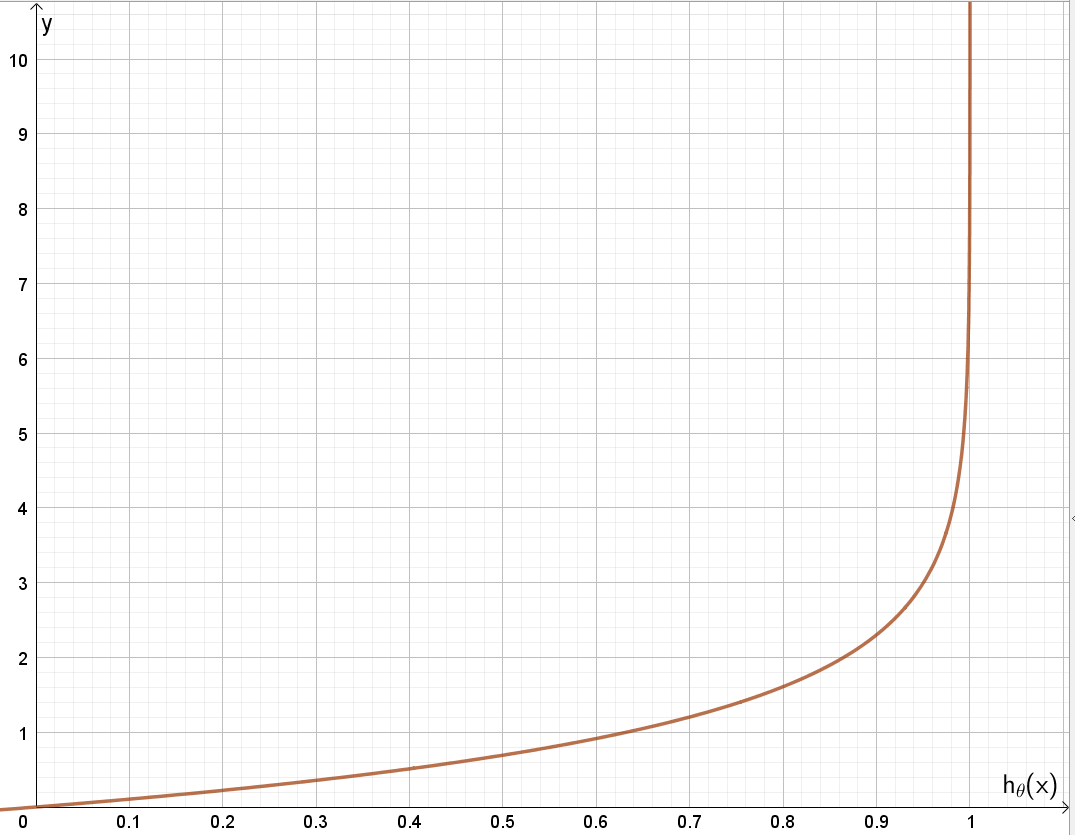
\includegraphics[scale=.75]{Abbildungen/Logistische_Regression_5}}
\caption{Implementierung Python}
\label{figure}
\end{figure}
%
\begin{figure}[hpt]
\centering
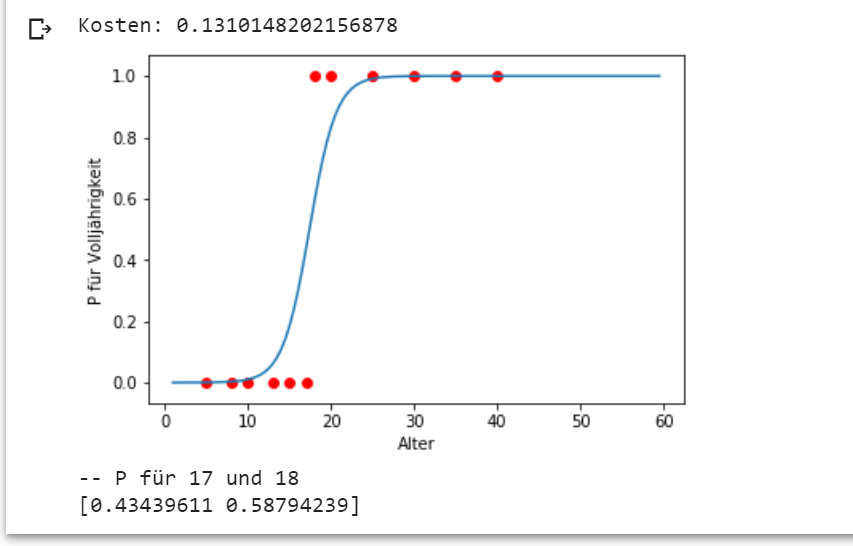
\includegraphics[scale=.99]{Abbildungen/Logistische_Regression_Python_2}
%\subfigure[$y=1$]{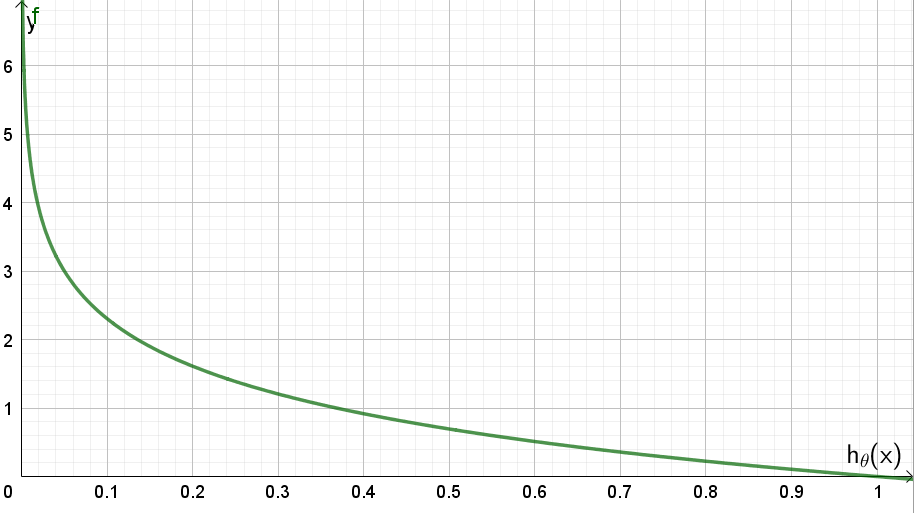
\includegraphics[scale=.75]{Abbildungen/Logistische_Regression_4}}
%\subfigure[$y=0$]{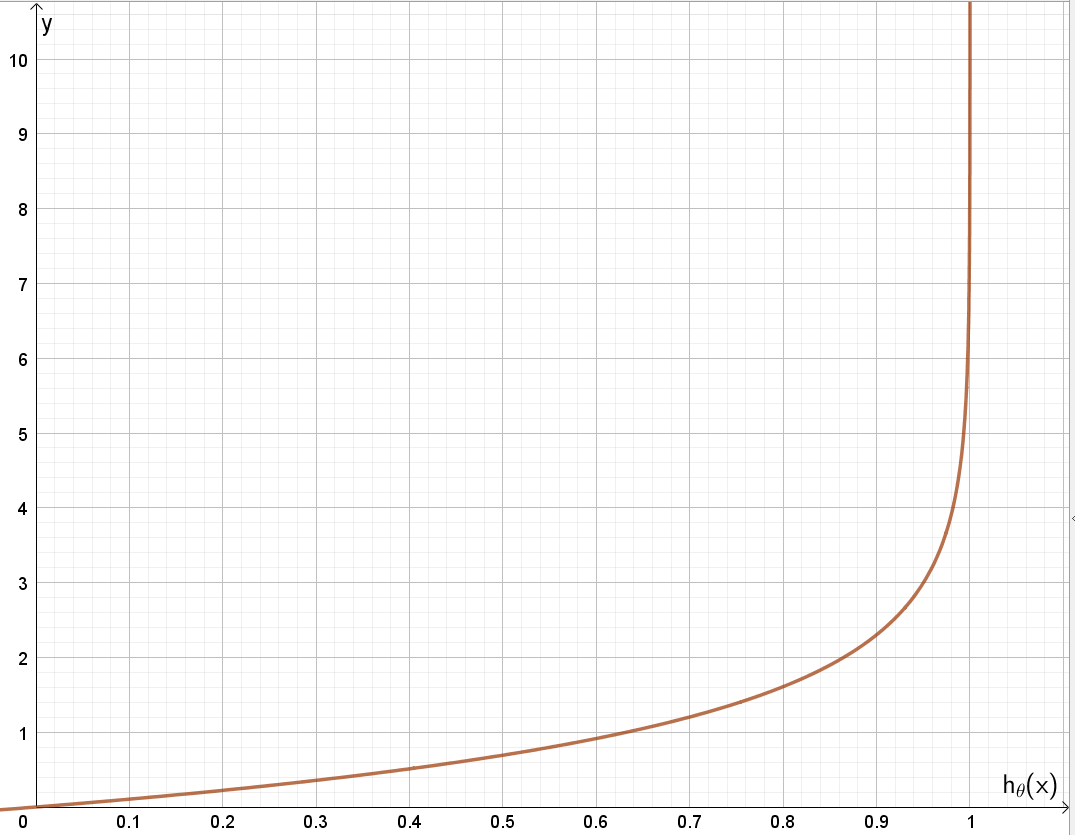
\includegraphics[scale=.75]{Abbildungen/Logistische_Regression_5}}
\caption{Ergebnisse Ausführung}
\label{figure}
\end{figure}
% Neuronale Netze
\chapter{Deep Learning}
\section{Neuronale Netzwerke}
Neuronale Netzwerke werden seit den 60'er Jahren des letzten Jahrhunderts erforscht. Schon immer hat den Menschen die Funktionsweise des biologischen Gehirns fasziniert. Daher ist es naheliegend, das Modelle zur Simulation der Gehirnfunktionalität erstellt wurden. Basierend auf den Erkenntnissen der biochemischen und bioelektrischen Vorgänge zwischen Nervenzellen wurden mathematische Modelle entwickelt, die derartige Netze abbilden. Die Forschung erhofft sich den Durchbruch zu einer generellen künstlichen Intelligenz (General Artificial Intelligence, GAI), die durch die Fortschritte in der Hardwareentwicklung, der Verbesserung von Algorithmen und durch den wirtschaftlichen Ansporn durch Anwendungen begründet werden. Neuronale Netzwerke sind sehr flexibel einsetzbar. Mittels eines Neuronalen Netzwerkes können sowohl diskrete Werte als auch verschiedenste Klassifikationen berechnet werden. Anwendungen dienen allgemein der Bilderkennung, der Vorhersage zeitdiskreter Werte zum Beispiel im Finanzbereich, der Sprachanalyse und vielem mehr. Unzählige Anwendungen etwa auf Smartphones wie Bilderkennung, Bildfilter, Fehlerkorrektur, personalisierte Werbung basieren auf Neuronalen Netzen.
\footnote{Andrew Ng- YouTube Video- Lecture 8.1 — Neural Networks Representation | Non Linear Hypotheses}
\newpage
\section{Aufbau eines Neuronalen Netzes}
Grundlegend  bestehen neuronale Netze aus schichtartig angeordneten Netzwerkknoten, den Neuronen, die Informationen also Werte enthalten und verarbeiten. An den äußeren Grenzen besteht das Netz aus einer Eingabe- und einer Ausgabeschicht (Input-, Outputlayer). Die Eingabeschicht enthält die zu verarbeitenden Daten $x_{i,j} \in X$, die Ausgabeschicht enthält die ermittelten Ergebniswerte $y_{i,k}$, mit $i$ als Anzahl der Datensätze, $j$ Anzahl der Eingabe- und $k$ Anzahl der Ausgabewerte. Die Anzahl der Eingabewerte pro Datensatz weicht in der Regel von der Anzahl der Ausgabewerte ab. Zwischen Eingabe- und Ausgabeschicht befindet sich eine Blackbox, die eine oder mehrere versteckte Zwischenschichten (Hiddenlayer) enthält.
\footnote{Jannis Seemann- Udemy Kurs Deep Learning verstehen: Entwickle Neuronale Netze in Python- Section 10- Wie ist ein Neuronales Netz aufgebaut?}
\\\\ 
Versteckt bezieht sich dabei auf die Sichtbarkeit der Werte innerhalb von Anwendungen, da der Nutzer des Netzwerks nur an den Eingabe und Ausgabewerten interessiert ist. Sind alle Neuronen einer Schicht mit der folgenden Schicht untereinander verbunden spricht man von einem Fully Connected Network. Die Anzahl der Zwischenschichten stellt die Tiefe des Netzes dar. Ab einer nicht näher definierten Tiefe spricht man vom Deep-Learning. Die Anzahl der Neuronen und Layer ist theoretisch unendlich. In der Praxis sind diese jedoch vor allem durch den benötigten Rechenaufwand (Hardware, Zeit) begrenzt.
\footnote{3Blue1Brown- YouTube Video- But what is a Neuronal Network? | Deep learning, chapter 1}

%
\begin{figure}[h!]
\centering
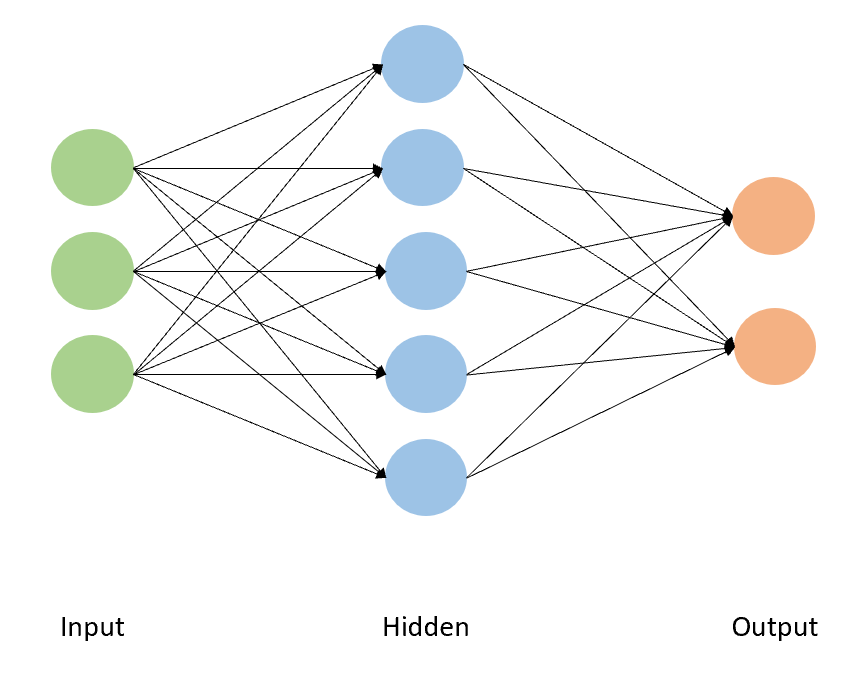
\includegraphics[scale=.65]{Abbildungen/Neuronale_Netze_00}
\caption{``Fully-Connected'' Neuronales Netz}
\label{figure}
\end{figure}
\newpage
Der Informationsfluss in dem Netzwerk erfolgt durch die vorwärtsgerichtete, gewichtete, schichtweise Weitergabe von Werten von der Eingabe- zur Ausgabeschicht. Dabei werden die Eingabewerte des Neurons wie bei der linearen Regression multipliziert und aufsummiert. Das Ergebnis führt mittels einer Aktivierungsfunktion, zum Beispiel der Sigmoidfunktion, im positiven Fall zur Weiterleitung des Wertes als Eingangswert an die nächste Schicht. Die Erwartung an das Netzwerk ist es, mathematische Strukturen durch Optimierung der Wichtungen im Netzwerk zu ermitteln. Damit wird umgangssprachlich das Lernen des Netzwerkes beschrieben.
\footnote{Jannis Seemann- Udemy Kurs Deep Learning verstehen: Entwickle Neuronale Netze in  Python- Wie machen wir mit einem Neuronen Netz eine Vorhersage}
%\newpage
Einen visuellen Einblick in die Funktionsweise kann man experimentell in Googles ``Tensorflow Spielwiese''
\footnote{\url{https://playground.tensorflow.org/}}
 und beispielhaft in Abbildung 4.2 erhalten.
%
\begin{figure}[h!]
\centering
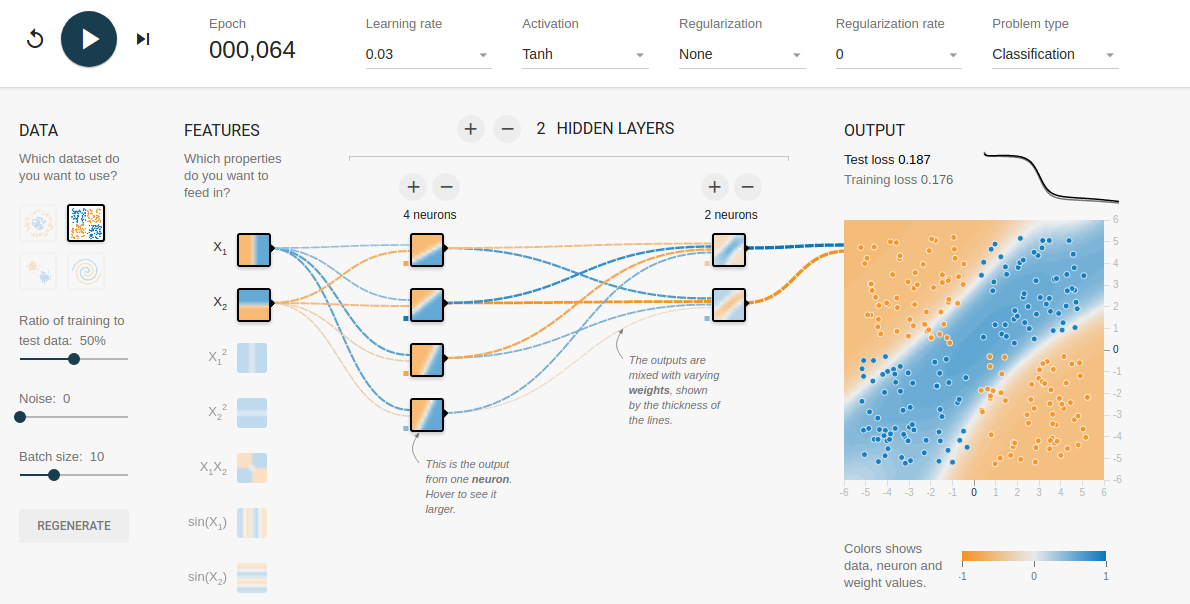
\includegraphics[scale=.3]{Abbildungen/Neuronale_Netze_1}
\caption{Informationsfluss Darstellung in Google Lab}
\label{figure}
\end{figure}
\\\\
Die Abbildung 4.3 stellt ein einfaches Neuron dar. Die Kanten zwischen den Knoten des Netzes sind die Wichtungen $\theta_{i}$ wobei $\theta_{0}$ ein spezieller Hyperparameter zur Verzerrung (Bias-Wert) ist, dem wie in der linearen Regression beschrieben ein $x_0=1$ zugeordnet wird. Die hier dargestellte Neuronenvariante verwendet die Sigmoid Funktion wie in der logistischen Regression, andere Funktionen zum Beispiel tanh, softmax oder relu verfügen über spezielle Eigenschaften und werden ebenso in Neuronalen Netzen eingesetzt. Somit kann ein Neuronales Netz auch als eine Matrix von Elementen der logistischen Regression angesehen werden.\\
%
\begin{figure}[h]
\centering
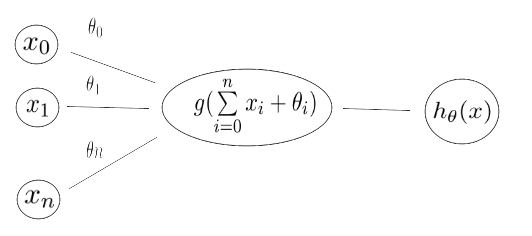
\includegraphics[scale=.64]{Abbildungen/Neuronale_Netze_2}
\caption{Einfaches Neuron mit Sigmoid-Aktivierung}
\label{figure}
\end{figure}
\\\\  
\section{Backpropagation}
Auch für die Neuronalen Netze existieren Kostenfunktionen, die optimiert werden müssen. Intuitiv ist anhand der vorgestellten, kleinen Neuronalen Netze deren komplexe Struktur erkennbar. Eine vollständige Herleitung würde daher den Rahmen der Facharbeit sprengen. Im wesentlichen besteht die verbreitete Methode der Backpropagation aus der bereits bekannten Optimierung durch das Gradientenabstiegsverfahren. Dabei muss in einem Netzwerk nicht nur die partielle Ableitung, also die Optimierung der Parameter pro Neuron (Knoten) erfolgen, sondern auch der Einfluss also das Gewicht des jeweiligen Neurons auf das Ausgabeergebnis berücksichtigt werden. Die einzelnen Wichtungen werden daher rückwärts von der Ausgabeschicht durch das gesamte Netzwerk pro Schicht zu einander ins Verhältnis gesetzt und nach den bekannten Schema optimiert. Für das algorithmische Vorgehen und die Ausrichtung der Hardware auf Matrizen- und Vektoroperationen ist diese Konstellation sehr geeignet. Für das menschliche Verständnis der mathematischen Formeln sind jedoch gute Kenntnisse der Notation komplexer Matrizenoperationen unabdingbar.\footnote{Jannis Seemann- Udemy Kurs Deep Learning verstehen: Entwickle Neuronale Netze in Python- Section 11- Intuition: Backpropagation}
\newpage
\section{Programmierbeispiel}
Die Programmierung eines einfachen Neuronalen Netzes erfolgt, natürlich komplexer, analog der bisherigen Beispiele. Zur Demonstration der Anwendbarkeit wurde ein vorab trainiertes Netzwerk von Tensorflow per Javascript in eine HTML Datei importiert, so dass auf der Seite eingebundene Bilder klassifiziert werden können. In der Abbildung 4.3 ist der recht kurze Quellcode dargestellt.
\footnote{Roland Schwaiger, Joachim Steinwendner, ``Neuronale Netze programmieren mit Python'', 2019 E-Book, Rheinwerk Computing Verlag}
%\newpage
%
\begin{figure}[h]
\centering
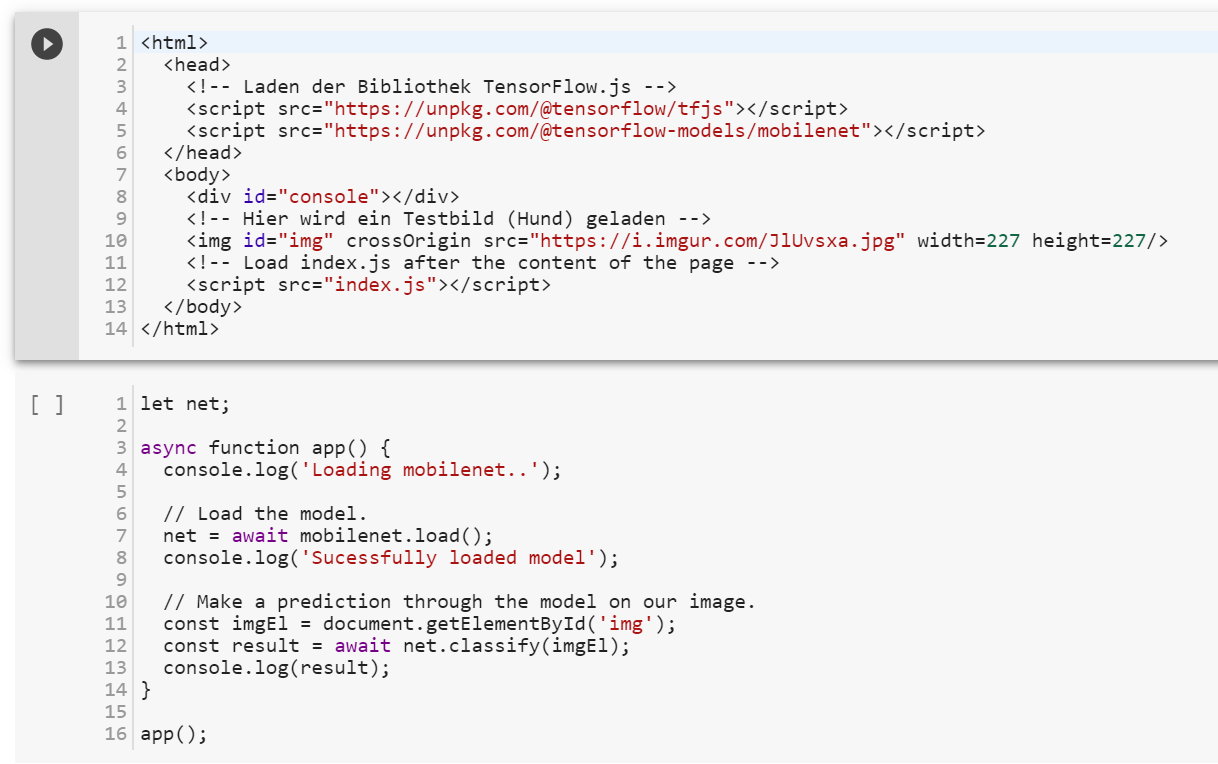
\includegraphics[scale=.84]{Abbildungen/Neuronale_Netze_3}
\caption{Bildklassifizierung Implementierung}
\label{figure}
\end{figure}
\newpage
Die Abbildung 4.4 bildet die HTML Seite mit dem Testbild ab (links). Die Konsole rechts zeigt die drei Klassifizierungsvorschläge des Netzwerks als Tags inklusive der berechneten Wahrscheinlichkeiten.\\
%
\begin{figure}[h]
\centering
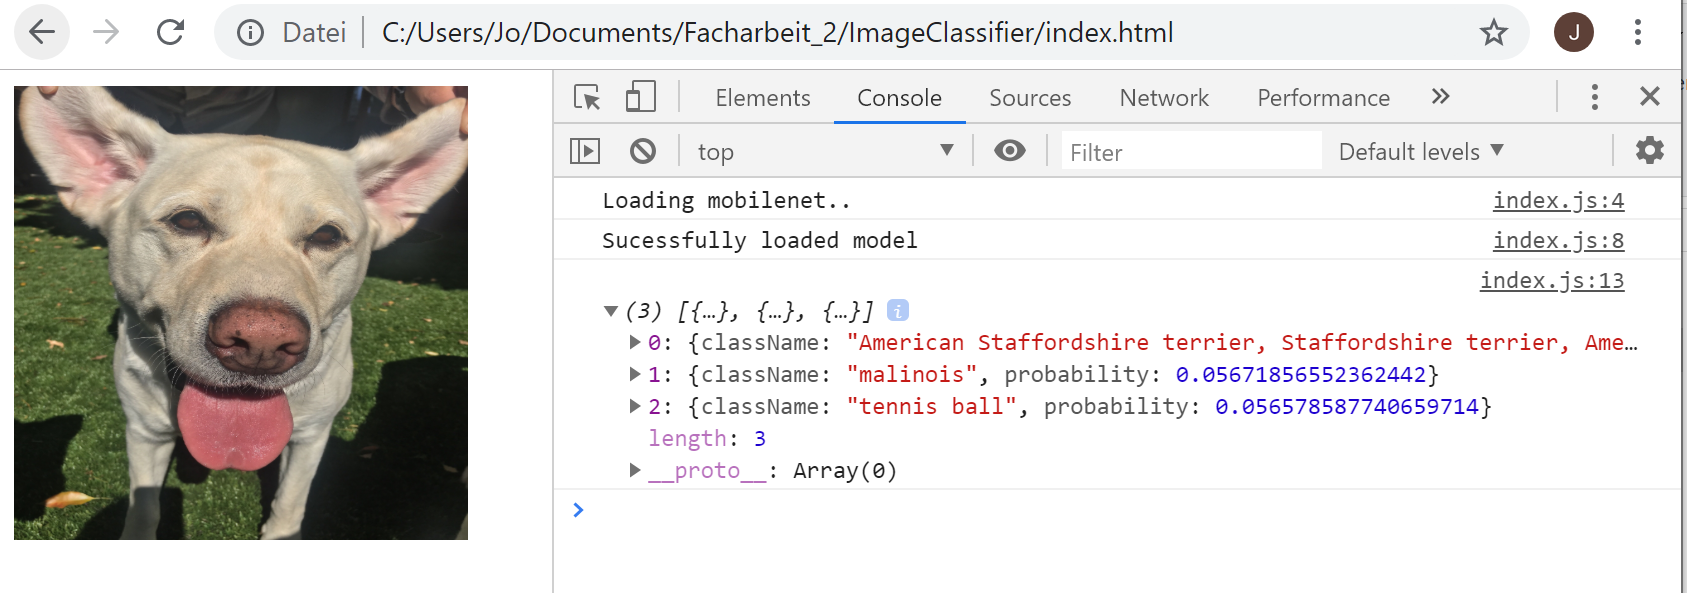
\includegraphics[scale=.54]{Abbildungen/Neuronale_Netze_4}
\caption{Ausführung Bildklassifizierung im Browser}
\label{figure}
\end{figure}
\\\\  

 
% Zusammenfassung
\chapter{Zusammenfassung}
Die Facharbeit sollte die mathematischen Grundlagen des Maschine-/ Deep-Learning unter der Berücksichtigung des Stoffes der Sekundarstufe II vorstellen. Die Wahl der einzelnen Algorithmen und Verfahren wurde von einfachen, intuitiven Lösungen zu den komplizierteren Modellen entwickelt. Die vielfältigen Voraussetzungen zum Beispiel bei der Aufarbeitung der Daten für ``echte'' Probleme,  kompliziertere und speziellere Methoden (K-NN, Random-Forrest, usw.), die Optimierung von Hyperparametern wie der Learningrate sowie in der Schule nicht gelehrte Verfahren zum Beispiel die partielle Ableitung von Matrizen konnten daher nicht weiter betrachtet werden.
Die Anwendung und Theorie dieses spannenden Gebietes wird zukünftig vielleicht selbstverständlich Teil des gymnasialen Schulstoffes, so wie es heute der CAS-Taschenrechner ist. Der beigefügte Python-Code dient nur unterstützend dem Verständnis des Textes und ist eng an die vorgestellten algorithmischen Vorgehen angelehnt. Für effizientere Lösungen wird daher auf entsprechende Bibliotheken verwiesen (Keras, Tensorflow, DL4J), in denen auch mit spezielleren Funktionen als den hier vorgestellten experimentiert werden kann.
Die KI wird in Zukunft unser Leben nachhaltig verändern. Dabei werden unzählige, heute noch einfache Algorithmen durch vernetzte und vielleicht durch eine Meta-KI entwickelte Algorithmen ersetzt. Durch die Konzentration gewaltiger Rechenkraft könnten einzelne Unternehmen generelle KI-Systeme erschaffen, die den Turing-Test bestehen und somit in der Interaktion mit Menschen von diesen nicht mehr als KI, sondern als Mensch wahrgenommen werden. Auf dem Weg dahin sind aber viele technische und auch ethische Probleme zu lösen. Wie jede Technologie bietet auch die KI eine Chance zur Verbesserung des Lebens der Menschheit (Lösung wichtiger Probleme z.B. Klima, Gesundheit, Nahrung) oder zu deren Verderben (Militäranwendungen zur autonomen Kriegsführung). Daher ist es wichtig, dass die Politik in Europa rechtzeitig Einfluss auf autokratisch regierte Länder und Großunternehmen nimmt und selbst in diesem Technologiefeld nicht zurückfällt.\newline
Für die Erstellung dieser Arbeit wurde das Textsatzusystem LaTeX, das Mathesystem GeoGebra, Python 3 und Google Colab verwendet, deren Vorstellung eine eigene Arbeit wert gewesen wäre. 
% Verwendete Quellen
\chapter{Quellen}
%Die Quellenlage ist vertrakt...
Internet Quellen:\newline
3Blue1Brown, ``Neuronal Networks'', abgerufen am 10.08.19 unter\\ \url{https://www.youtube.com/channel/UCYO_jab_esuFRV4b17AJtAw}
\\\\
Andrew Ng - ``Youtube Lectures Linear, Logistic Regression, Neuronal Networks'', abgerufen unter:\\ \url{https://www.youtube.com/channel/UC5zx8Owijmv-bbhAK6Z9apg}
\\\\
Andrew Ng - ``CS229 Lecture Notes'', abgerufen am 10.08.19 unter\\ \url{http://cs229.stanford.edu/notes/cs229-notes-deep_learning.pdf}
\\\\
Jannis Seemann - Udemy Kurs: ``Machine Learning von A-Z''
\\\\
Jannis Seemann - Udemy Kurs: ``Neuronale Netze in Python''
\\\\
Bücher:\newline
Arnfried Kemnitz, ``Mathematik zum Studienbeginn'', 9. Auflage, Vieweg + Teubner
\\\\
Roland Schwaiger, Joachim Steinwendner, ``Neuronale Netze programmieren mit Python'', 2019 E-Book, Rheinwerk Computing Verlag
\end{document}



